\begin{multicols}{2}
\chapter{Introduction}

Our group was given the task to design and implement an analog PID hotplate controller. This is the final report regarding our project. Here, we have broken down the device into 6 main subparts. 
\begin{itemize}
    \item Power Supply
    \item Zero crossing detector and Ramp generator
    \item DC PWM controller
    \item PID error controller
    \item Sensor input interface
    \item Triac firing angle controller
\end{itemize}
We will further discuss these parts throughout the report.\\
The PID controlling mechanism is one of the best and widely used error-correcting methods with high efficiency when properly tuned. In this project, our main goal was to implement an analog-based PID temperature controller for a 220V AC 1KW hotplate controller with a firing angle control mechanism.
\begin{center}
    
    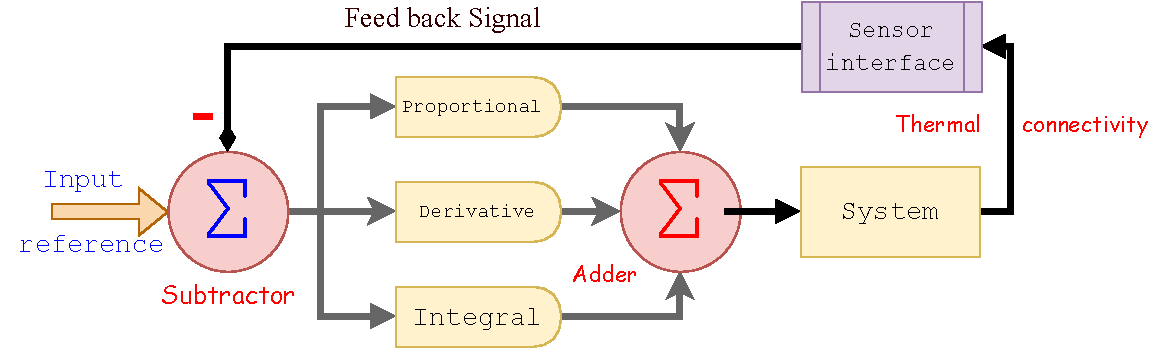
\includegraphics[width=0.5\textwidth]{Introduction/PiD .pdf}
    \captionof{figure}{PID controller}
    
\end{center}
Here we can observe a block diagram of the PID control mechanism we implement. Feedback is taken from the temperature sensor.

The real time temperature is read using a RTD PT100 temperature sensor. The PT100 is an industrial grade temperature sensor with a wide temperature range. The sensor changes the resistivity with the temperature. It changes in an linear manner so the PT100 was a suitable option.
\begin{center}
    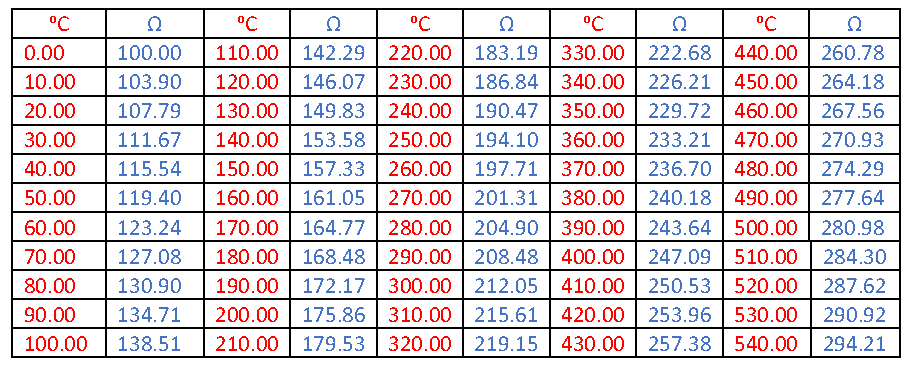
\includegraphics[width=0.5\textwidth]{Introduction/pt100 range updated-cropped.pdf}
    \captionof{figure}{PT100 resistivity look up table}
    
\end{center}

The AC current is controlled by a TRIAC and to separate AC and DC parts we are implementing a MOC3021 optocoupler. Also, 12V center taped stepdown transformer is used to obtain the appropriate voltages.

{\let\clearpage\relax \chapter{Method}}
%\section{Steps of the Project}

Since simulating and implementing analog systems is complex, we created our system sequentially. In this section, it will be shown, the order in which these separated sections interconnect and their behaviour.

\begin{minipage}{0.5\textwidth}
\centering

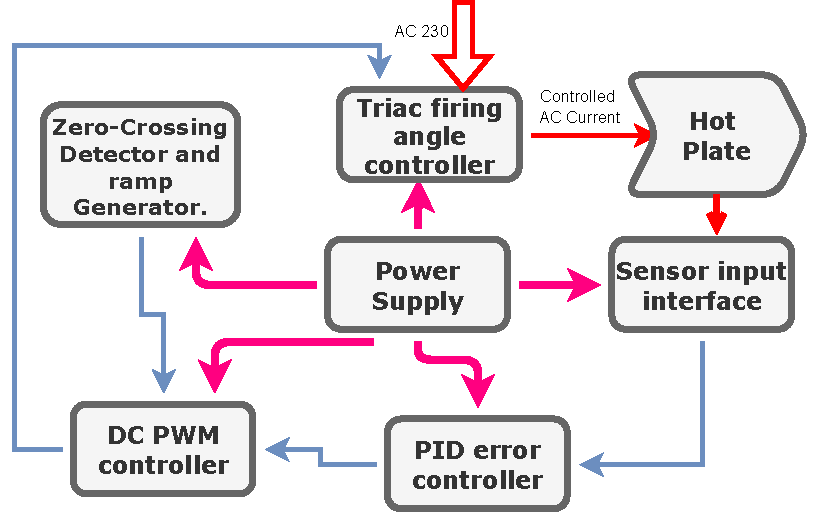
\includegraphics[width=\textwidth]{Method/Block diagram.pdf}
\captionof{figure}{Block Diagram}
\end{minipage}

\section{Power Supply}
For our project we need +12V ,-12V , Phase synchronized 100Hz rectified signal and a common ground. We have to take the power from the same source as the hotplate power source. We have to match the phase of the generated PWM signal with the AC power source of the hotplate in order to get the correct firing angle. Using 240V(RMS) to 12V(RMS) step-down center tapped transformer as the power input. This power supply have 4 subparts. 
\begin{itemize}[leftmargin=*]
    \item Using a rectifier bridge, we will take a full wave rectified voltage from top and center terminals. This will be used as the input to the zero crossing detector.
    \item To get +12V DC voltage, we will directly feed +12V AC trough a diode to take the half rectified wave. Using a 7812 voltage regulator with 2 capacitors, the half rectified wave will be stabilized. Since the 12V terminal is used a lot, we have implemented two of these.
    \item Since we are using 741 OP-Amps, we also need -12V power supply to utilize them. By using the same method as +12V circuit, and a 7912 voltage regulator, using the 180$^{\circ}$ 12V AC bottom terminal, with the input as the half rectified wave rectifying the negative half cycles, we will get the -12V DC supply.
\end{itemize}
\begin{minipage}{0.45\textwidth}
\centering
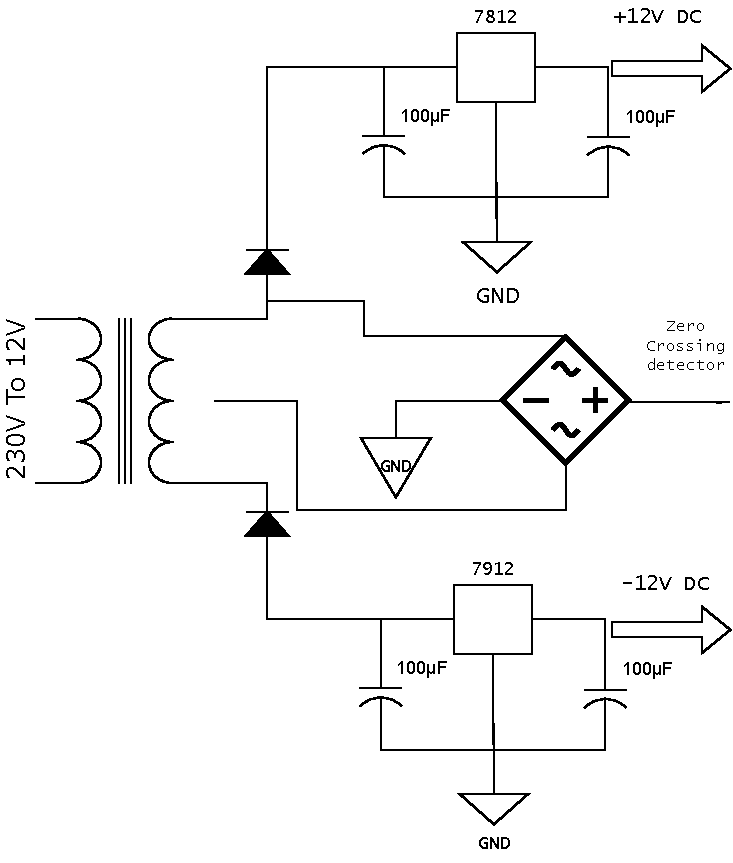
\includegraphics[width=\textwidth]{Method/Power supply.pdf}
\captionof{figure}{Power supply unit}
\end{minipage}

The current that can be supplied by the transformer is limited to 300mA. The single 7812 and 7912 voltage regulators can handle up to 1A. To stabilize and to smooth-up the output voltage wave form we will use 100$\mu F$ electrolyte capacitors.

\section{Zero-Crossing detector and the ramp generator }
To control the firing angle, we need to modulate the width of a square wave. Also, since we have to use a triac with the ability to control both half cycles of the sine wave, we need a square wave with twice the frequency(100Hz). Also, the phases should be matched.

To archive this task, we are taking the following steps.

\subsection{ Zero Crossing region detector}

Using the rectified wave as the inverting input and a forward biased diode as the non-inverting input, we have implemented a zero crossing area detector for the 0.7V region in the rectified wave. The LM339 comparator is powered with +12V DC and the Ground voltage. 
When the inverting input is smaller than 0.7V, which we consider as the zero crossing area, the comparator will hold the positive saturation voltage (12V) in that time .Once the inverting input exceed the 0.7V value, the comparator will give the negative saturation voltage, which is ground voltage.

\begin{minipage}{0.45\textwidth}
\centering
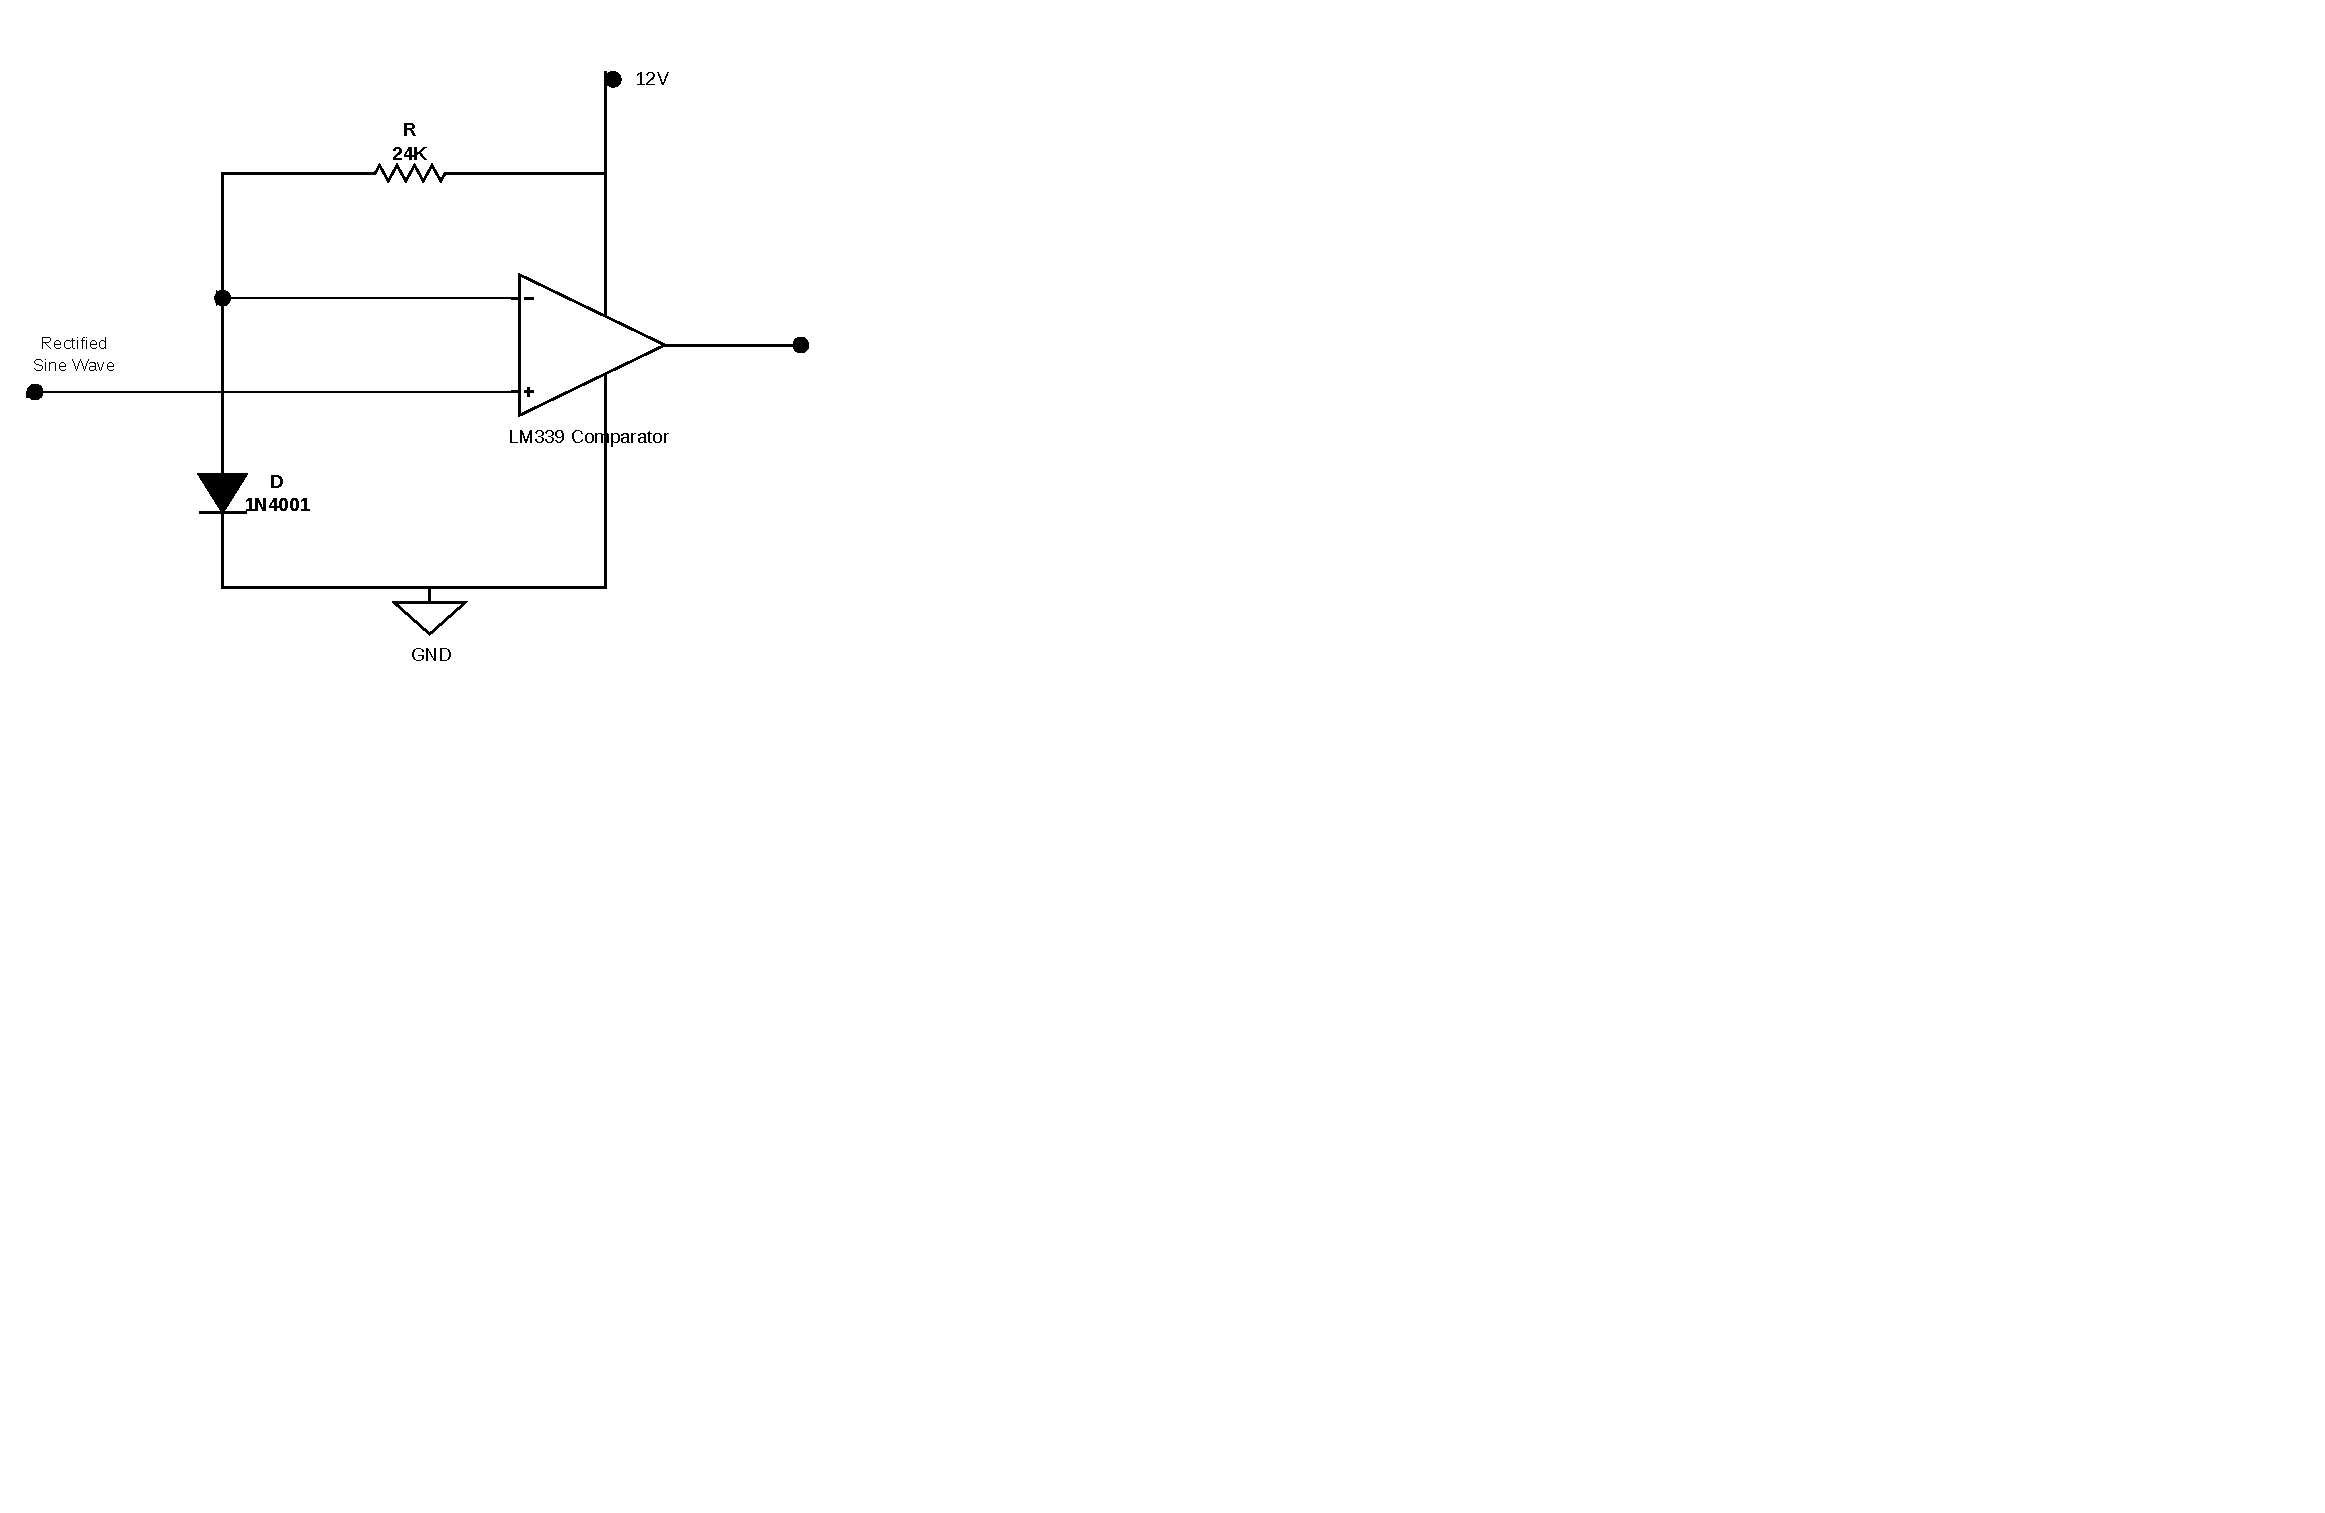
\includegraphics[width=\textwidth]{Method/Ze_Area Pluse.drawio.pdf}
\captionof{figure}{Zero crossing region detector}
\end{minipage}

\begin{minipage}{0.45\textwidth}
\centering
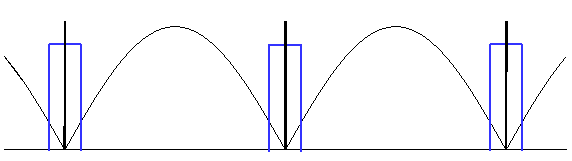
\includegraphics[width=\textwidth]{Method/Zero-ramp function.pdf}
\captionof{figure}{Zero crossing region graph}
\end{minipage}

The LM339 chip contains 4 separate comparators inside it. We will be only using two of them throughout the project.


\begin{minipage}{0.45\textwidth}
\centering
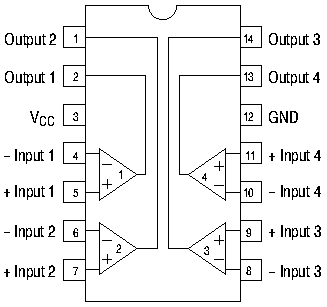
\includegraphics[width=0.6\textwidth]{Method/LM339.pdf}
\captionof{figure}{LM339 Quad comparators}
\end{minipage}

 
 %To archive this, we are using a forward biased diode voltage as the non inverting input and feed the rectified wave as the inverting input. By rectifying the 50Hz AC wave, we can get a signal with 100Hz frequency. To archive this we are using a LM339 Quad differential comparator. It is a single power supply unit. The circuit only use a single comparator.
 
\subsection{Ramp generator}
After recognizing the zero crossing region, next we have to generate the relevant PWM signal. Inorder to get the intended width, first we generate a ramp which can be matched with the phase of the AC signal. To match the phases, we will use the square wave we generated earlier. 


\begin{minipage}{0.45\textwidth}
\centering
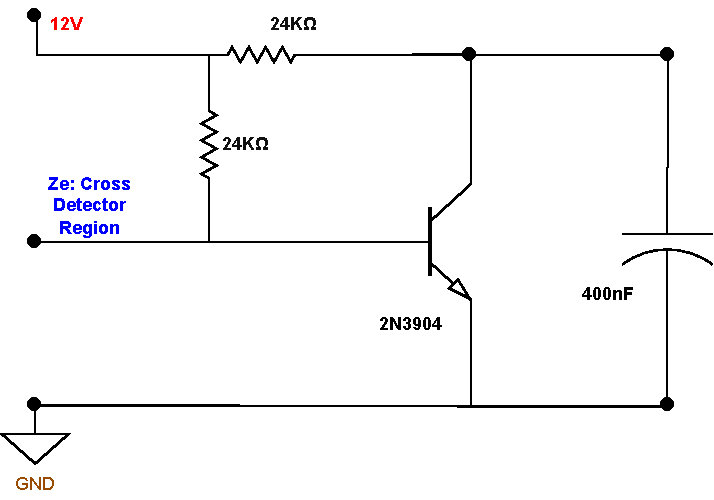
\includegraphics[width=\textwidth]{Method/Ramp gen cropped.pdf}
\captionof{figure}{Ramp Generator Circuit}
\end{minipage}

This Resistor - Capacitor is one of the most simple ramp generating circuit. The RC ramp generator will use a  capacitor to generate the ramp. A parallel connected BJT will be used to provide a discharge path for the capacitor. Once the pulse is present at the base terminal, the BJT will be transferred to the saturation state and closing the circuit to provide a discharge path. The capacitor will be discharged till it become the saturation $V_{CE}=0.2 \; V$. Once the base voltage is 0V, the BJT will be transferred to the cut off region. So the current will flow through the capacitor and charge it. The voltage waveform across the capacitor will provide a ramp.

\begin{minipage}{0.45\textwidth}
\centering
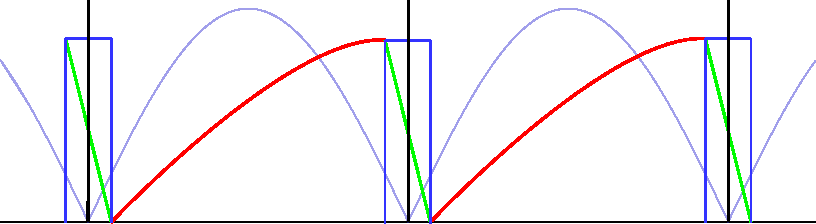
\includegraphics[width=\textwidth]{Method/Zero-ramp function with ramp.pdf}
\captionof{figure}{Zero crossing with ramp graph}
\end{minipage}

\section{PWM controller}
To control the firing angle, we need a square wave to trigger the optocoupler. Using another comparator inside the LM339 chip, we are comparing the ramp wave we generated previously with a reference input. This reference voltage will be provided by the PID error control circuit. 

\begin{minipage}{0.45\textwidth}
\centering
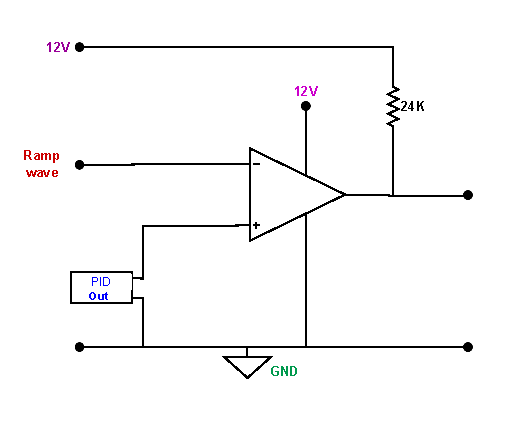
\includegraphics[width=\textwidth]{Method/PWM width controller circuit.pdf}
\captionof{figure}{PWM Generation Circuit}
\end{minipage}

The PID unit will provide a calculated voltage level. The comparator will then generate a PWM signal with the proper duty cycle. The higher the voltage, the lower the duty cycle will be.


\begin{minipage}{0.45\textwidth}
\centering
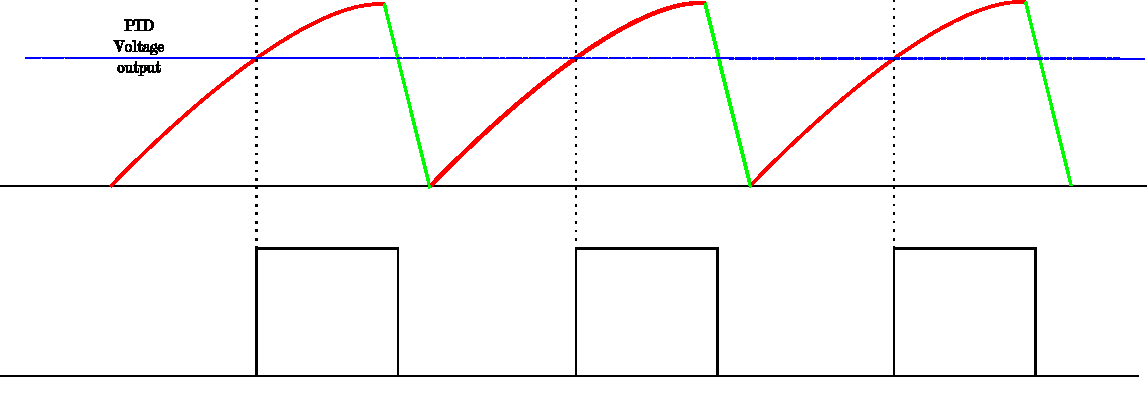
\includegraphics[width=\textwidth]{Method/PWM Genration from ramp graph.pdf}
\captionof{figure}{PWM Generation Graph}
\end{minipage}

\begin{minipage}{0.45\textwidth}
\centering
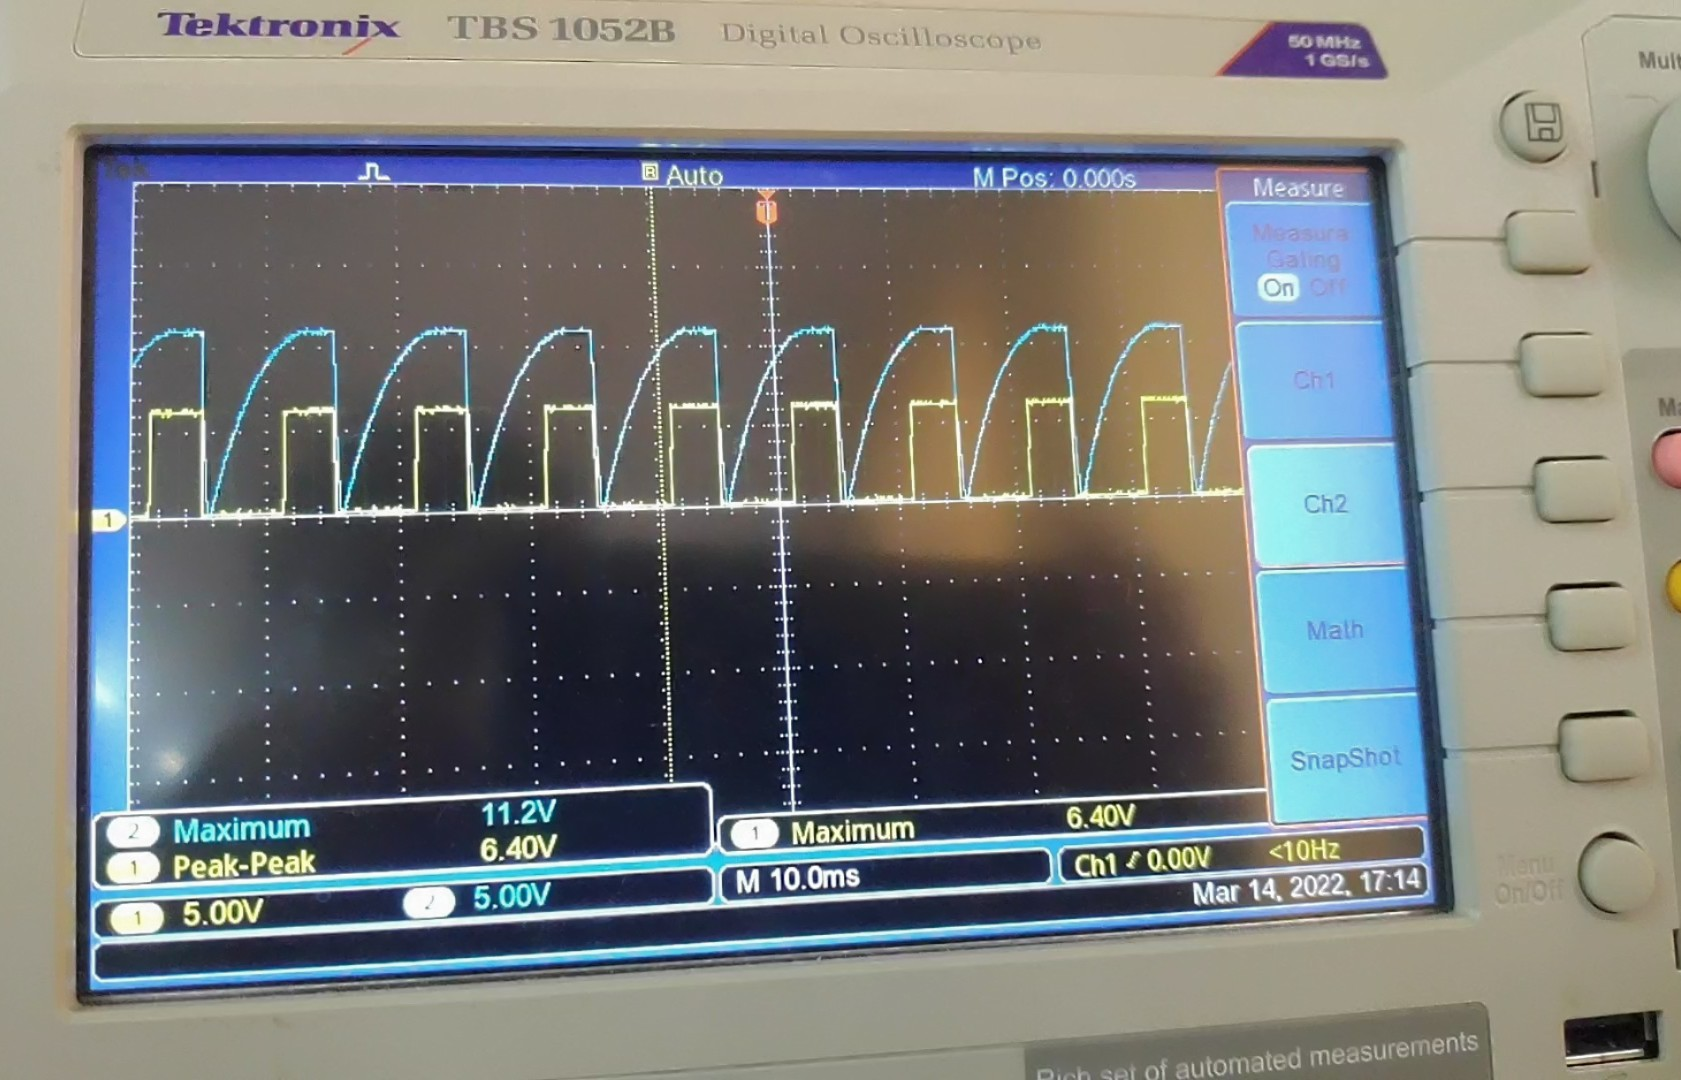
\includegraphics[width=\textwidth]{ramp 2.jpg}
\captionof{figure}{PWM Generation Graph Oscilloscope}
\end{minipage}

\section{Sensor input interface}
The PT100 temperature sensor changes it's resistivity with temperature. The job of the sensor input interface is to provide a constant current and give a temperature reading with a voltage level. Since high currents dissipate high power,
$$P \; = \; I^2 \times R$$
We must provide a small current through the sensor. Because, if the sensor is heating from the dissipated power, we will not get a proper temperature reading. So a constant current source of $1mA$ is provided to the sensor and then the voltage output will be re-scaled to the required range of $0-12V$ linearly. Following steps will be used to archive this task.

\subsection{PT100}
Pt100 temperature sensor is a high precision sensor with fast response time. Basically this temperature sensor maps the temperature to resistance. The mapping is mostly linear, and the relationship between temperature and the resistance can be represented by the following equation.

\resizebox{0.45\textwidth}{!}{
R =\begin{cases} 
    $R_0 ( 1 + AT + BT^2 + C( T - 100) T^3 )$ &  -200$^\circ$C\leq x\leq 0$^\circ$C \\
    $R_0 ( 1 + AT + BT^2 )$ &  0$^\circ$C\leq x\leq 800$^\circ$C \\
 \end{cases}
 }

Where,\\
$ A        = 3.9083 \times 10^-3 ^\circ C^{-1} \\
B        = -5.775 \times 10^-7 ^\circ C^{-2} \\
C        = -4.183 \times 10^-12 ^\circ C^{-3} \\
R_0 = 100\; \Omega$

\begin{minipage}{0.45\textwidth}
\centering
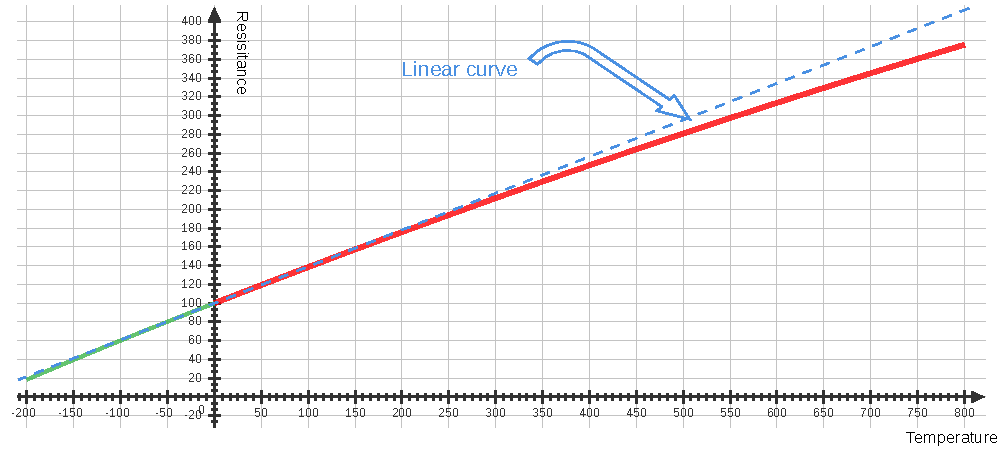
\includegraphics[width=\textwidth]{Method/pt100 curve.pdf}
\captionof{figure}{PT100 Curve}
\end{minipage}

The current from the constant current source will be feed to this sensor and the voltage drop will be feed to the instrumentation amplifier.

\subsection{Constant Current Source}

To provide a high precision small 1mA, we are using a improved Howland current pump with a buffer. The added buffer has high input impedance which will introduce a high output impedance to the constant current source. Higher the output impedance, better the stability of the current output. So compared with a version without the buffer, this model have better accuracy. The improved version provides the freedom to choose the gain value,

\begin{minipage}{0.45\textwidth}
\centering
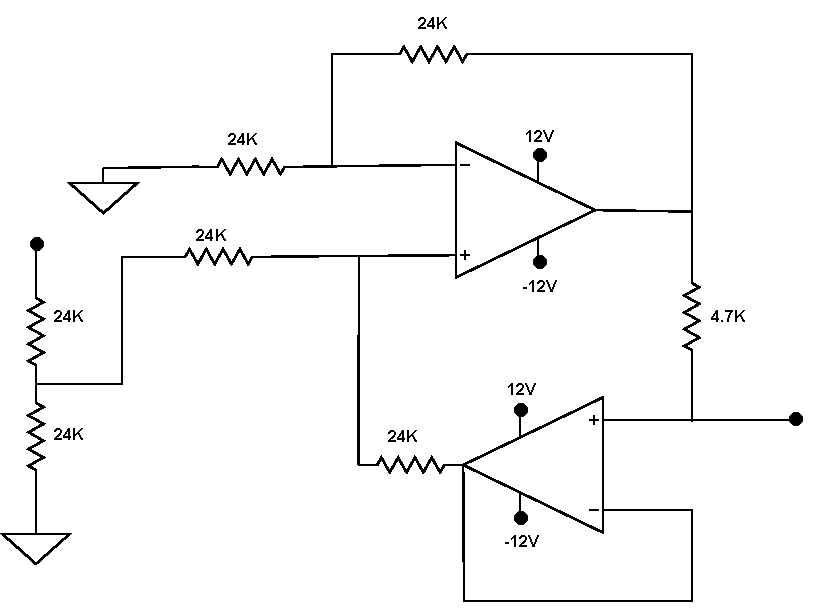
\includegraphics[width=\textwidth]{Method/Constant current.pdf}
\captionof{figure}{Improved Howland Current Pump}
\end{minipage}

$$Gain (G) = \frac{R2}{R1}$$

Also, it minimizes the error by removing the feedback current.

The output current can be calculated by the following equation.
$$I(output)=\frac{G \times (V_p - V_n)}{R_s}$$

%add the circuit    
Here the $Gain=1$. The $V_p =6V $ and $V_n =0V $. So the output current is\\ $I_{out}=\frac{6V}{4.7k\Omega}=1.2765mA$

But, the circuit does not provide a $V_{cc}$ of a 12V. also considering other non perfect issues, we get an actual current around $1.05mA$

\subsection{Instrumentation Amplifier}
Instrumentation amplifiers are usually used to amplify very small signals with, high accuracy. Here the voltage drop between the Pt100 will be in millivolts range.There are instrumentation amplifier ICs in the market. But they are expensive. Here Using 3 741 opamps, we have implemented an InAMP to get the voltage range into volts range.

\begin{minipage}{0.45\textwidth}
\centering
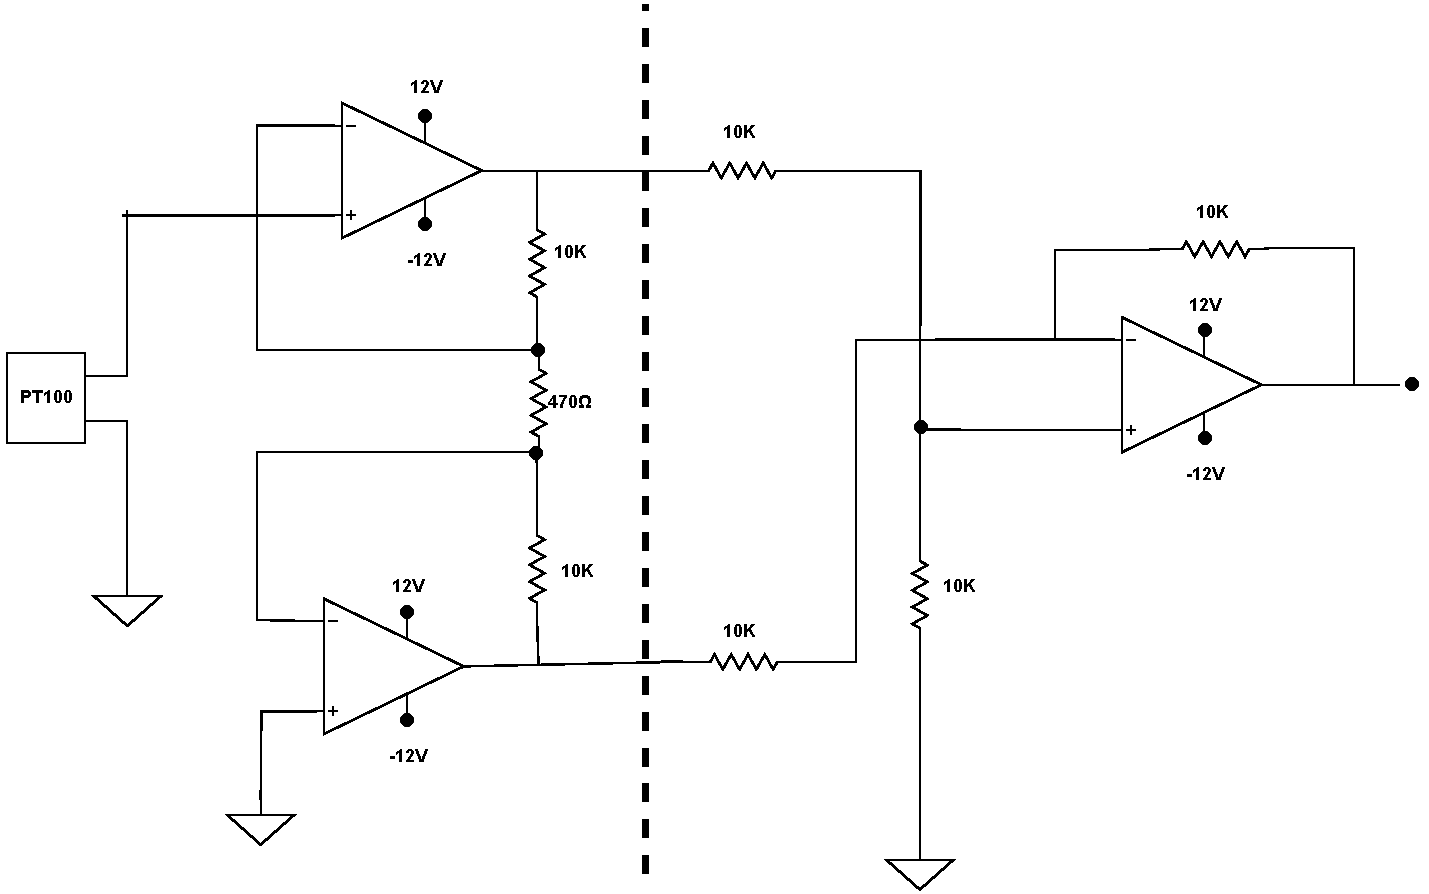
\includegraphics[width=\textwidth]{Method/ins.pdf}
\captionof{figure}{Instrumentation amplifier}
\end{minipage}

$$A_V=\frac{V_{out}}{V_{pt100}}=(1+ \frac{2R_1}{R_{gain}})\times \frac{R_3}{R_2}$$
$$ A_V = (1+ \frac{2\times 10k}{470})\times \frac{10k}{10k}$$
$$A_V=43.553$$

The circuit design have two stages. In the first stage, there are two buffer amplifiers. Once these two are connected, it provides a voltage follower. This will provide high input impedance. Which is ideal for a sensor voltage reading. Higher the input impedance, lower the effect on the sensor voltage output drop. 
Next step is a differential amplifier, it provides very low output impedance to the instrumentation amplifier. It will avoid the loading effect in the next stage of the sensor input interface.



\subsection{Voltage Scaling}
Since we are working with the voltage range of $-12V \; to \; +12V$, we are mapping the sensor output range to $0V\; to +12V$ range. Also, in our design we are considering the change in ambient temperature. The PT100 sensor have a resistance of 100$ \Omega$ at 0$^\circ C$. \\
In our design, at the ambient room temperature the reference input voltage will be 0V. So, in the PID error controlling, room temperature should be matched with 0V input. Also, since the room temperature does change with time and place, we have added a feature to fine tune this scaling circuit to suit any room temperature, by proving a potentieometer.

\begin{minipage}{0.45\textwidth}
\centering
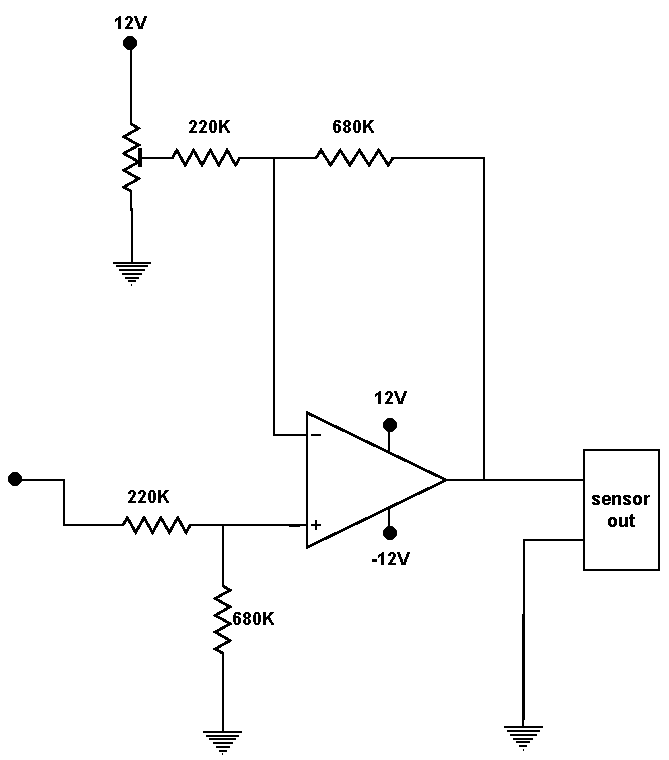
\includegraphics[width=\textwidth]{Method/Scalers.pdf}
\captionof{figure}{Voltage range changer}
\end{minipage}

To archive this, we have added an Op-amp differential amplifier with 741 Op-amp.
$$ V_{out} = \frac{R_3}{R_1}(V_2 - V_1)$$

This will re-scale the voltage in the following manner with,
$$y=m(x-c)$$

Since, $R_3=680k\Omega$ and $R_1=220k\Omega$
the voltage gets amplified 3.09,which is nearly 3 times.

\section{PID error controller}
 The Proportional-Integral-Derivative (PID) controller, is one of the most important part in this design. Considering that this is a hotplate temperature controller, the temperature change is actually not that rapid. But to optimize for any situation, we are implementing a PID error controlling mechanism. The reference voltage input and the scaled sensor voltage output will be compared and the system will determine a proper output voltage using the proportional, integral and the derivative parts in the system. Then the separate outputs will be added using an opamp adder with unity amplification. 

As we mentioned earlier, the PWM generator will generate a pwm with a smaller duty cycle for a higher voltage output. But when the error is high, when we actually need a higher PWM duty cycle, it will give a  smaller PWM. So we need to remap the voltage output of the adder. For that we are using a inverter. It will map negative outputs to zero, 0V to +12V and +12V to 0V.

\subsection{Proportional}
The most effective and the most basic part of the error controller is the proportional error controller. 

\begin{minipage}{0.45\textwidth}
\centering
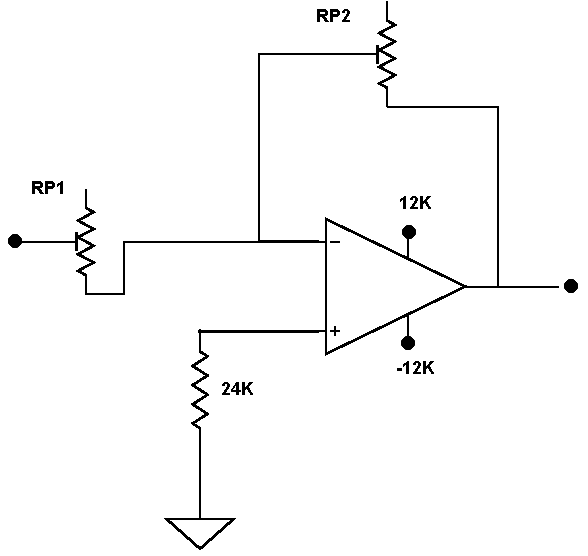
\includegraphics[width=\textwidth]{PID/P.pdf}
\captionof{figure}{P-Controller}

\end{minipage}

%diagram
$$V_{op} = -\frac{R_{P2}}{R_{P1}}\; V_{err}$$

Here we have implemented an inverting amplifier with a 741 op amp.
Given the error $e(t)$ we can write the characteristic equation as,
$$c(t)=K_p e(t)$$
As the equation suggests, the relationship between the error and the output is linear. 

The $K_p$ tends to react more quickly for a error and tends to gain a level faster. This will indeed increase the react time, but it can cause overshooting. Also increasing $K_p$ will help to reduce the steady state error.
\\

\begin{minipage}{0.45\textwidth}
\centering
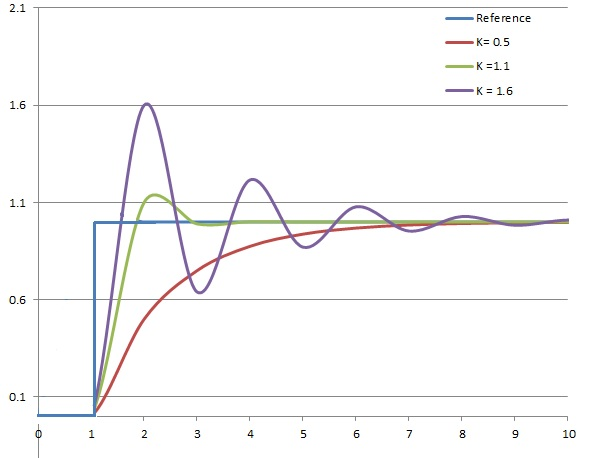
\includegraphics[width=\textwidth]{PID/PID_varyingP.jpg}
\captionof{figure}{Varying $K_p$}
\end{minipage}

\subsection{Integral}
The integral part of the error controller have bit slower response time. The philosophy behind the integral error control is that, deviations will be affected in proportion to the continuous cumulative sum of their magnitudes.
\begin{minipage}{0.45\textwidth}
\centering
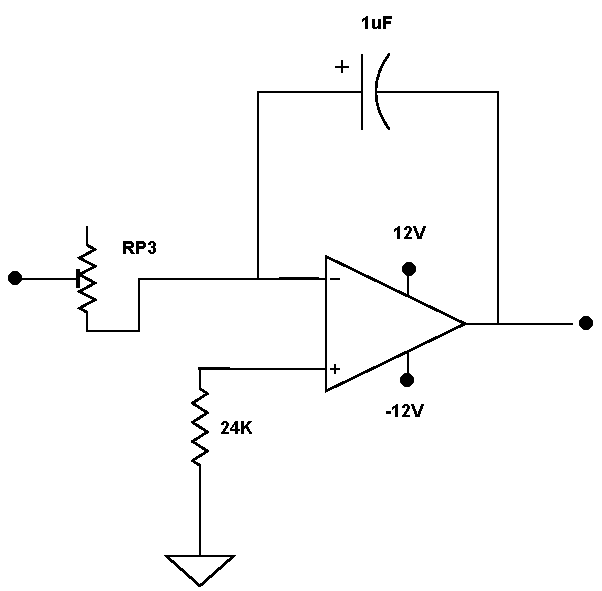
\includegraphics[width=\textwidth]{PID/I.pdf}
\captionof{figure}{I-Controller}
\end{minipage}
%diagram
$$V_{oi}=- \frac{1}{R_{P3} C} \int V_{err} d t  $$
Here we have implemented an integrator with a 741 op amp. The characteristic equation as follows,

$$c(t)=K_i\int e(t) d t$$

This term will tend to help reduce the steady state error. The downside of this term is that, it will make the output more oscillatory. This effect will be minimized by the proportional term. The circuit needs to be fine tuned to get the best result.


\begin{minipage}{0.45\textwidth}
\centering
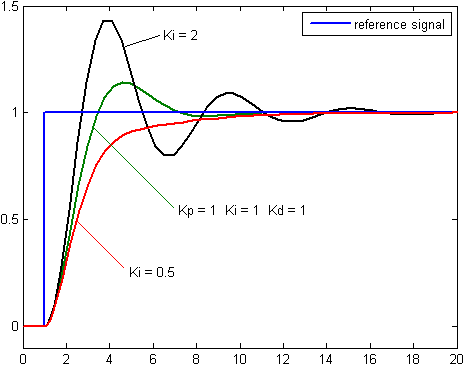
\includegraphics[width=\textwidth]{PID/Change_with_Ki.png}
\captionof{figure}{Varying $K_i$}
\end{minipage}

\subsection{Derivative}
The derivative part gives the error controller the ability to predict the error. It have little influence over a small change in the error. It will be  calculated by determining the slope of the error over time and taking a proportional gain over that error change rate.
%diagram
\begin{minipage}{0.45\textwidth}
\centering
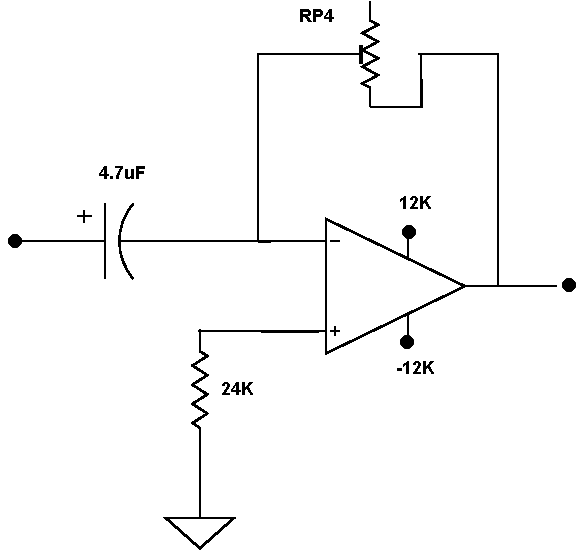
\includegraphics[width=\textwidth]{PID/D.pdf}
\captionof{figure}{D-Controller}
\end{minipage}

$$V_{od}=- R_{P4} C \frac{d V_{err}}{d t}$$
Here we have implemented a simple differentiator with a 741 op amp. The characteristic equation as follows,

$$V_{od}=K_d \frac{d e(t)}{d t}$$

The anticipation effect which is caused by the monitoring the slope tends to add damping effect to the system. And by doing so, it will reduce the overshooting effect. Rather than depending on only with the error magnitude, the derivative term will also consider the time frame.

\begin{minipage}{0.45\textwidth}
\centering
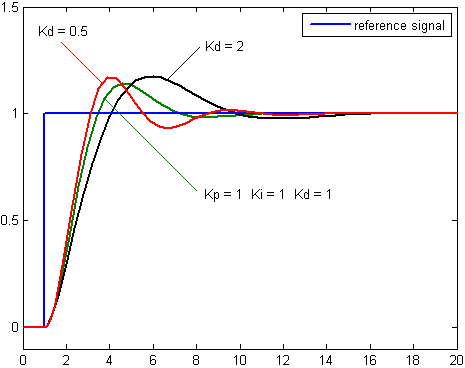
\includegraphics[width=\textwidth]{PID/Change_with_Kd.png}
\captionof{figure}{varying $K_d$ }
\end{minipage}

\subsection*{Overview}
We included potentiometer to tune our PID controlling system. After successfully completing all the subparts, we tested our product and using trial and error methods we fine tuned our PID controller.

\begin{minipage}{0.45\textwidth}
\centering
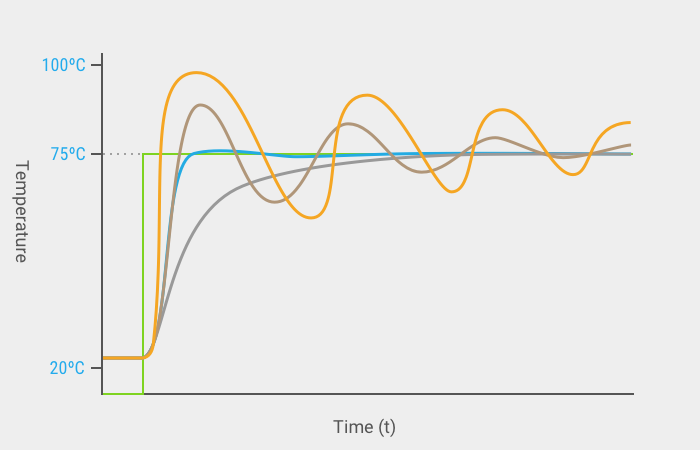
\includegraphics[width=\textwidth]{PID/PID_Master_Graph.png}
\captionof{figure}{PID controlling system }
\end{minipage}

\section{TRIAC firing angle controller}
The temperature controller is done by changing the Power of the supply voltage. To change power we need to change root square mean(RMS). In order to archive this task, we can either change the amplitude of the AC current wave form, or remove a certain part of the signal. Here we have implemented a circuit to change the firing angle and only let part of the wave pass through.

\begin{minipage}{0.45\textwidth}
\centering
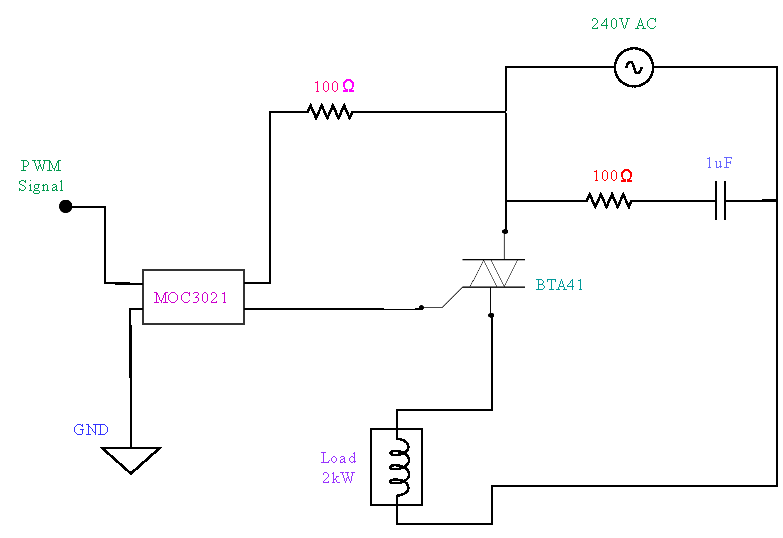
\includegraphics[width=\textwidth]{Method/Triac Cct.pdf}
\captionof{figure}{Firing Angle Controller Circuit }
\end{minipage}



As shown in the above diagram, we have implemented a optocoupler-triac circuit with a snubber circuit stabilizer.
The triac we used is a BTA41600B triac. It can handle upto 41A(rms) current and 600V(rms) voltage input given a proper heat dissipation method. We noticed that the triac heat up significantly while running a higher power rating devices. So we included a heat sink to address this issue. Also, the traic has zero crossing control. So once the gate gets triggerd, it will keep the gate open till the terminal currents become zero.

The MOC3021 optocouplers is triggered using the PID controlled PWM signal. We are only using it to isolate the AC current and to provide a triggering current to the triac gate.

To keep the internal mechanism of PWM genaration stable and not to draw current from that mechanism, we have implemented a voltage follower between the PWM signal output and the MOC3021 optoisolater. Once the internal diode is forward biased, the moc3021 will keep voltage drop around 1.4V .

\begin{minipage}{0.45\textwidth}
\centering
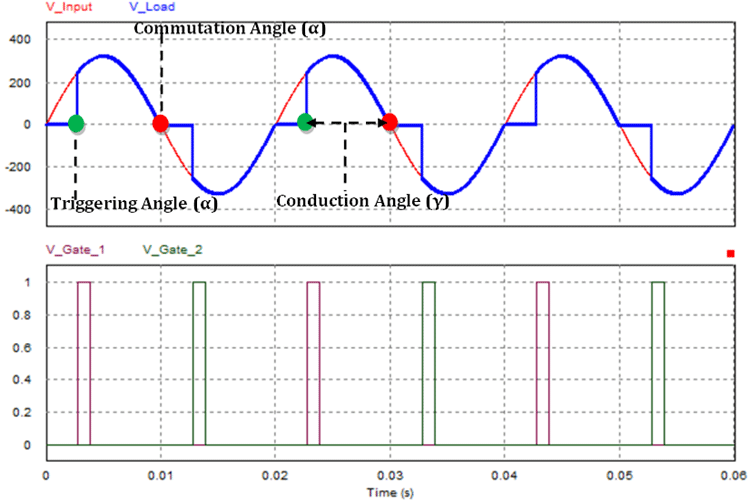
\includegraphics[width=\textwidth]{trig angle.png}
\captionof{figure}{Traic Firings }
\end{minipage}

\begin{minipage}{0.45\textwidth}
\centering
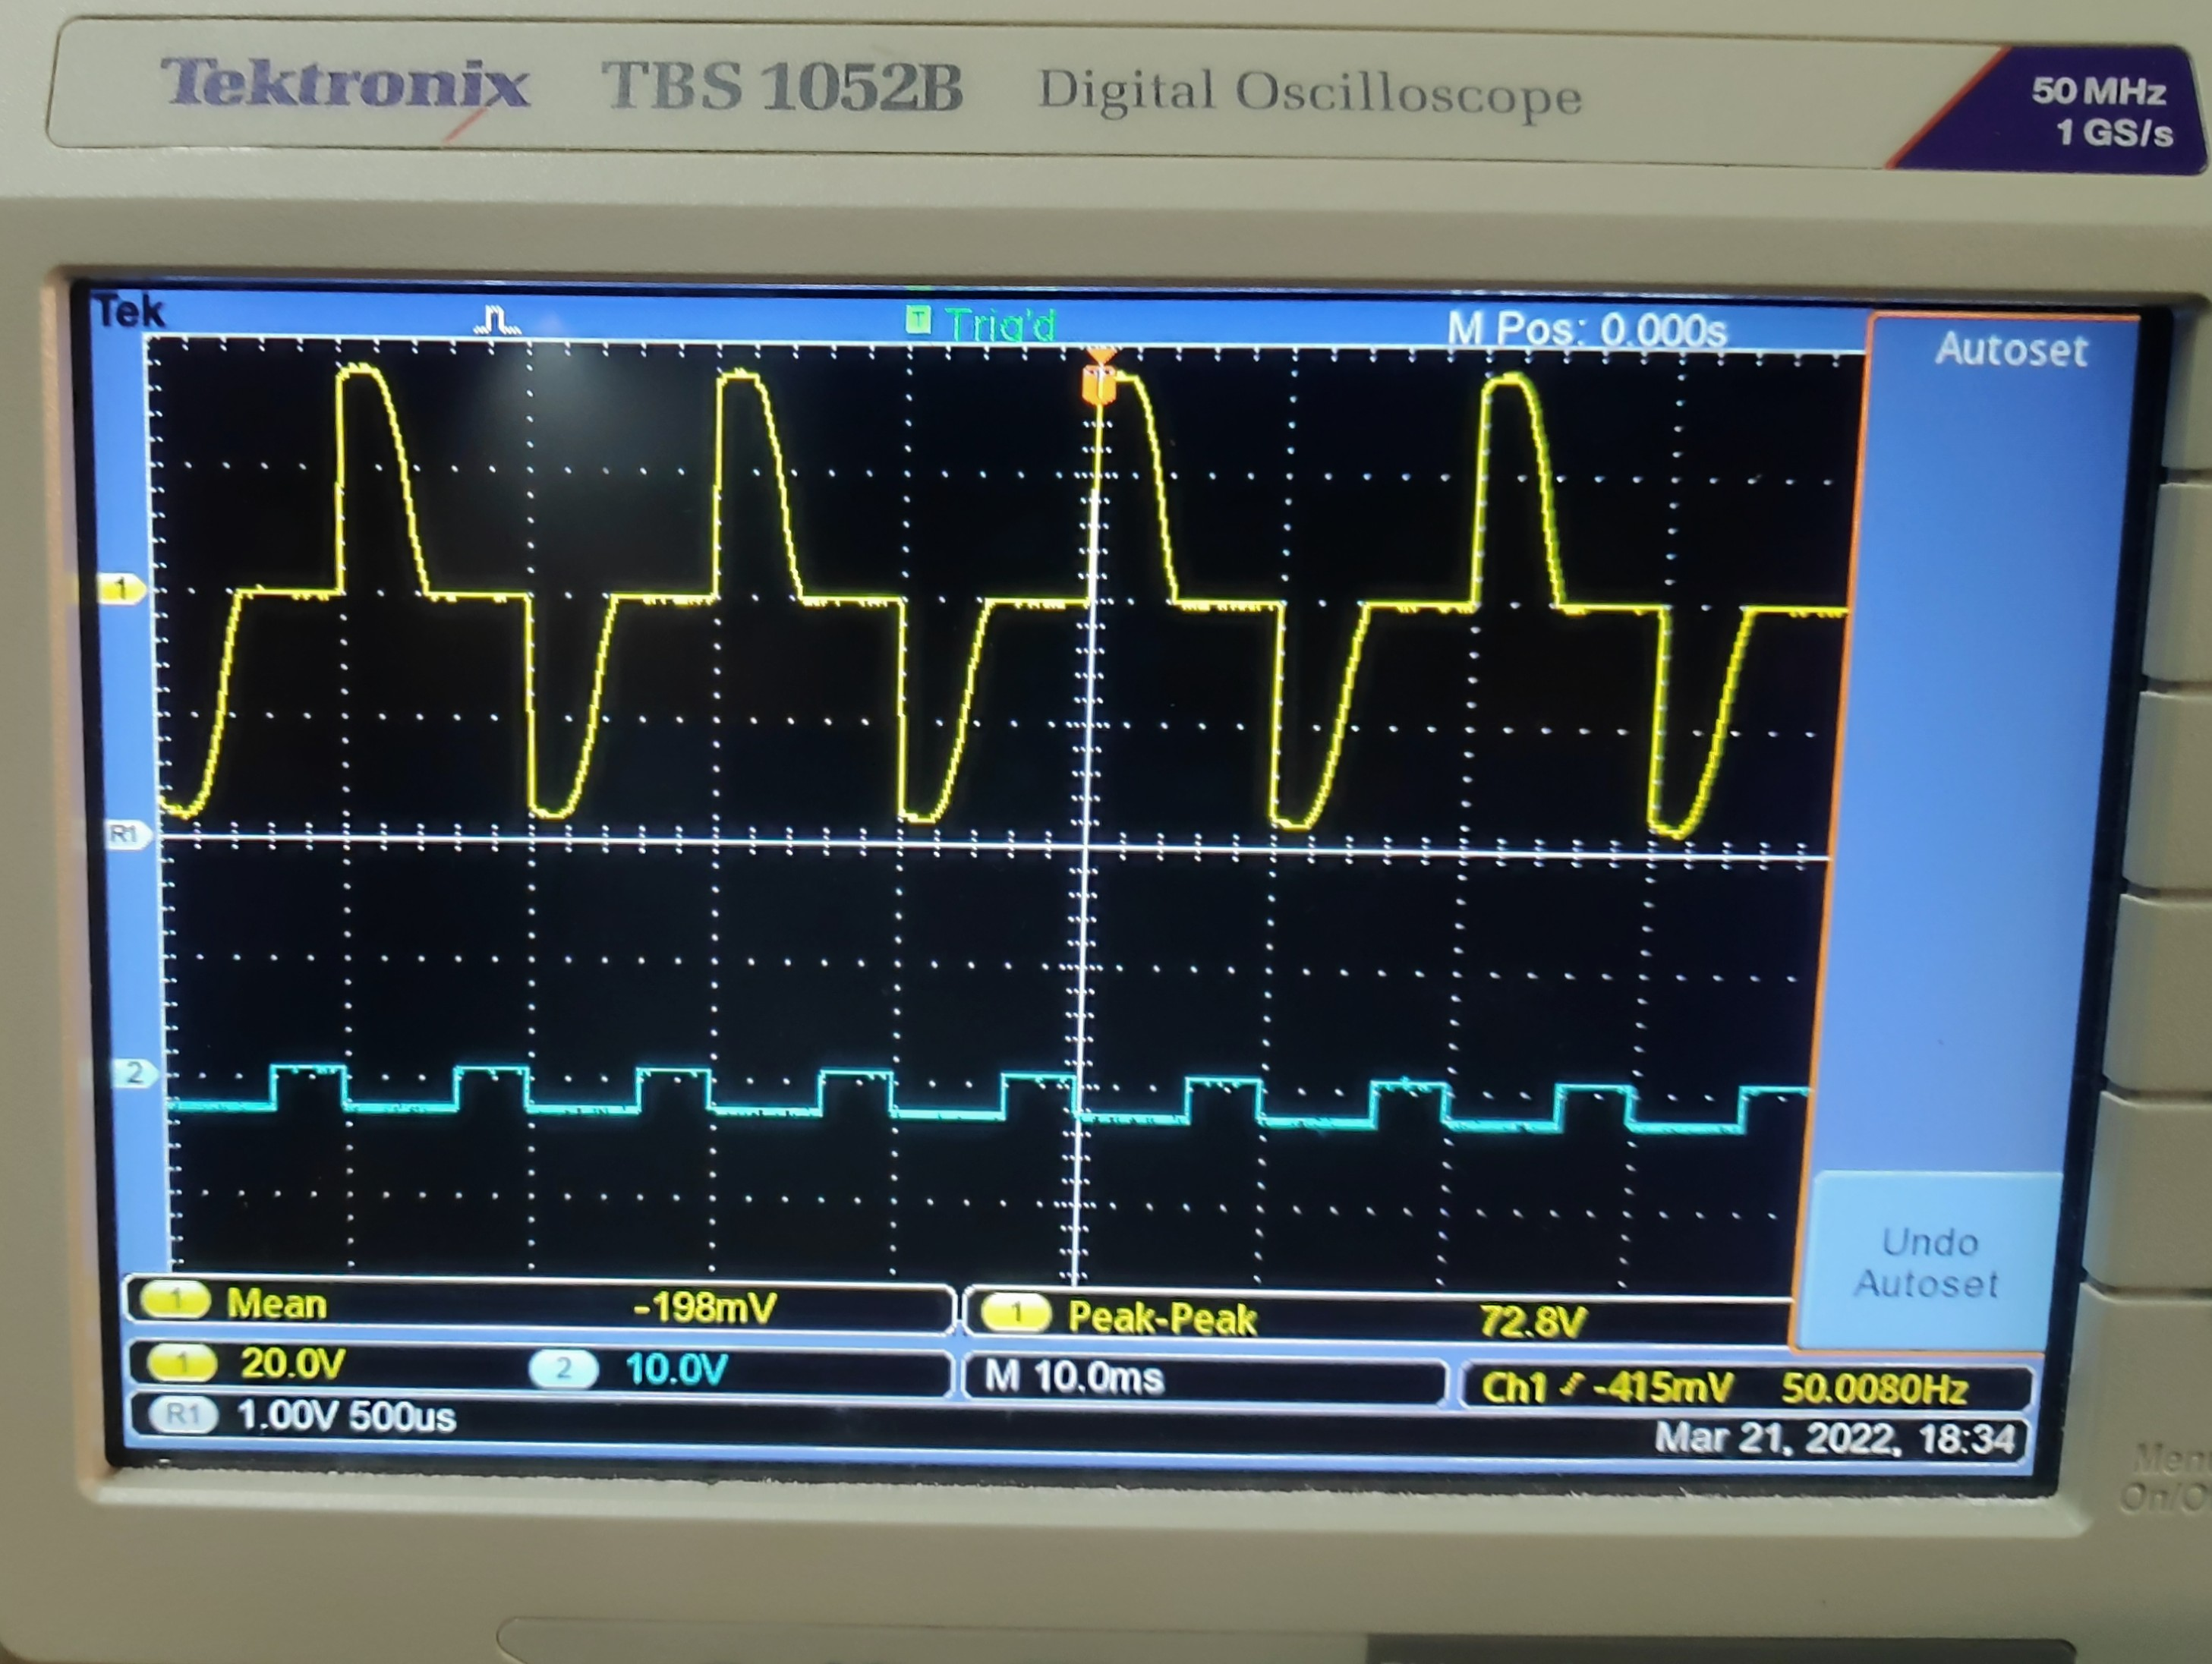
\includegraphics[width=\textwidth]{Triac oc.jpg}
\captionof{figure}{Traic Firings Oscilloscope image}
\end{minipage}

The RC snubber circuit which lies parallel to the load and the tirac mechanism is often used for inductive loads. In this case, our hotplate could be used with an inductive device. So to limit the slope of the reapplied voltage and to ensure right TRIAC turn-off, we are using the above mentioned snubber circuit.

{\let\clearpage\relax \chapter{Results}}
First, we created our circuits in breadboards,After successfully combining all the subparts, we observed some voltage drops. So to fix these problems, we added voltage followers along. And after that, we printed our circuit board. 
The printed circuit board contained all other subparts other than the triac circuit and an op-amp inverter.

The printed circuit board was 2 layer copper board. The triac circuit was soldered on a dot board. To allow high current to pass, we added 10A routing copper-cables to connect pins.

To test our circuit we used a 1500W water heater and 1000W water heater separately and parallelly as well. We observed that the PID controller is working properly and the system stabilizes after some time. We were not able to find a proper thermometer to map inputs properly with the stabilized temperature output. We were only able to identify 5 to 6 number of temperature input points. 

\begin{minipage}{0.45\textwidth}
\centering
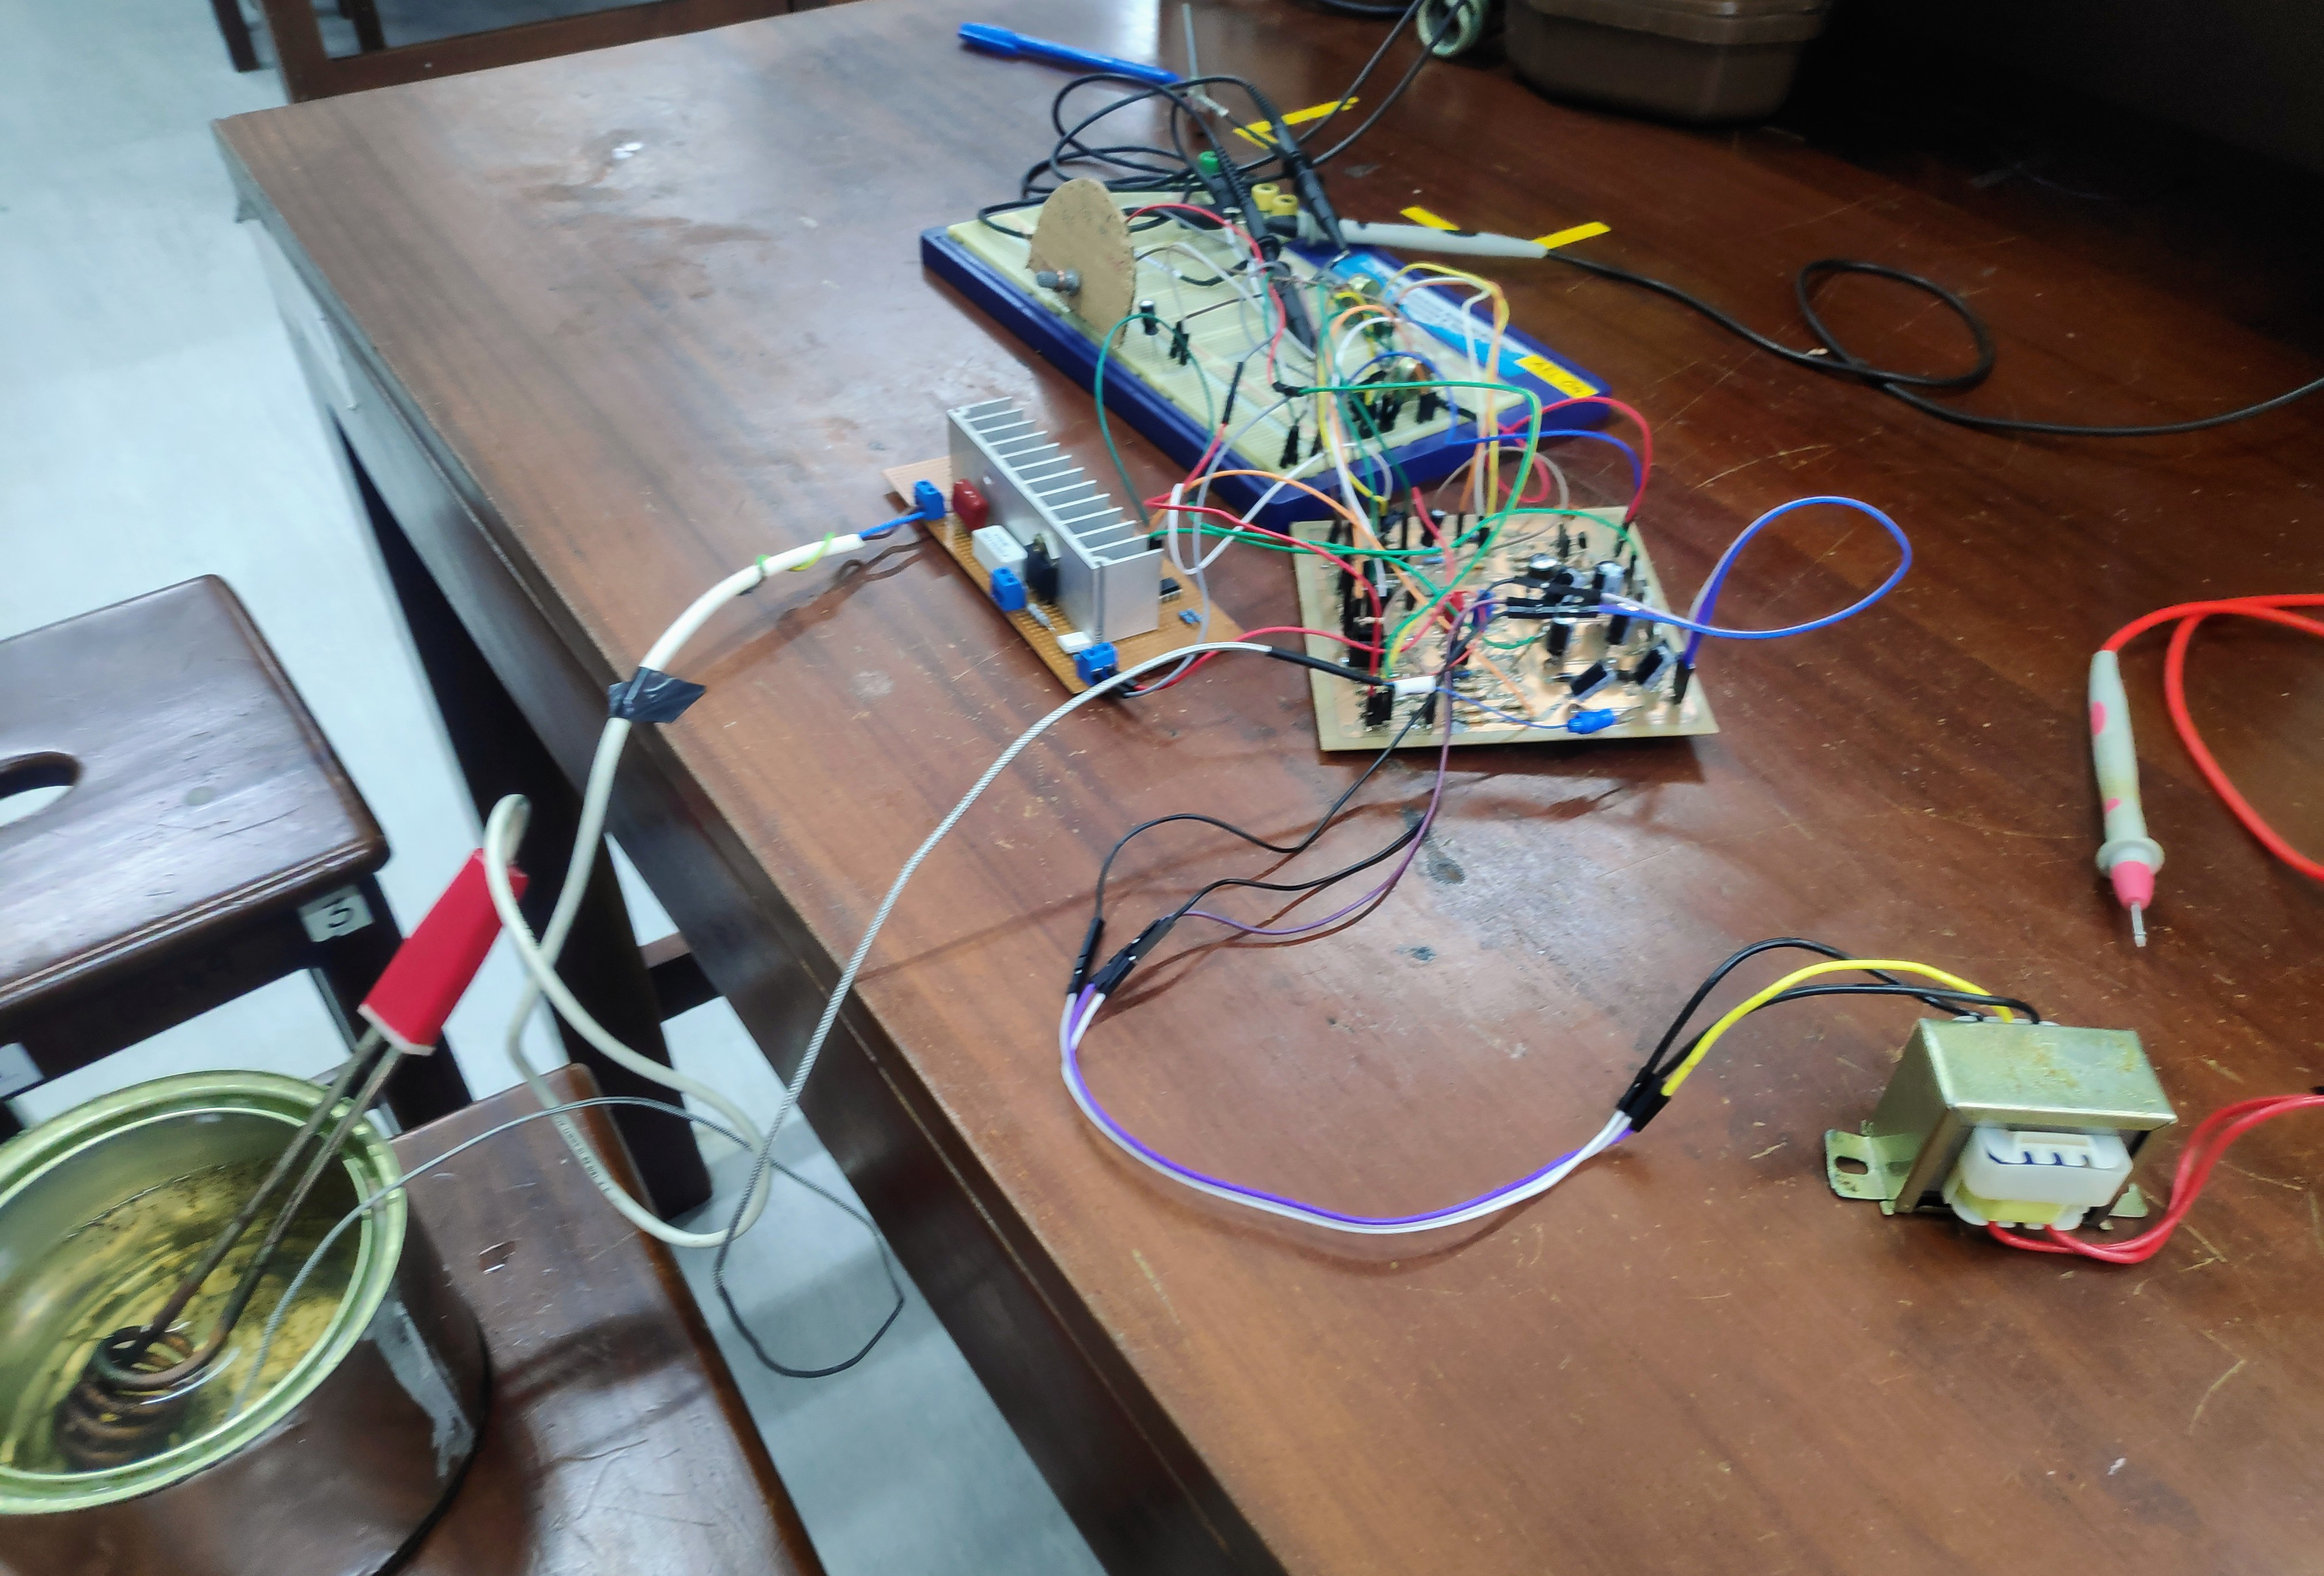
\includegraphics[width=\textwidth]{PCB fabricated/Final.jpg}
\captionof{figure}{Evaluation Setup}
\end{minipage}

\begin{minipage}{0.45\textwidth}
\centering
\includegraphics[width=\textwidth]{PCB fabricated/triac_cct.jpg}
\captionof{figure}{Triac Circuit}
\end{minipage}

\begin{minipage}{0.45\textwidth}
\centering
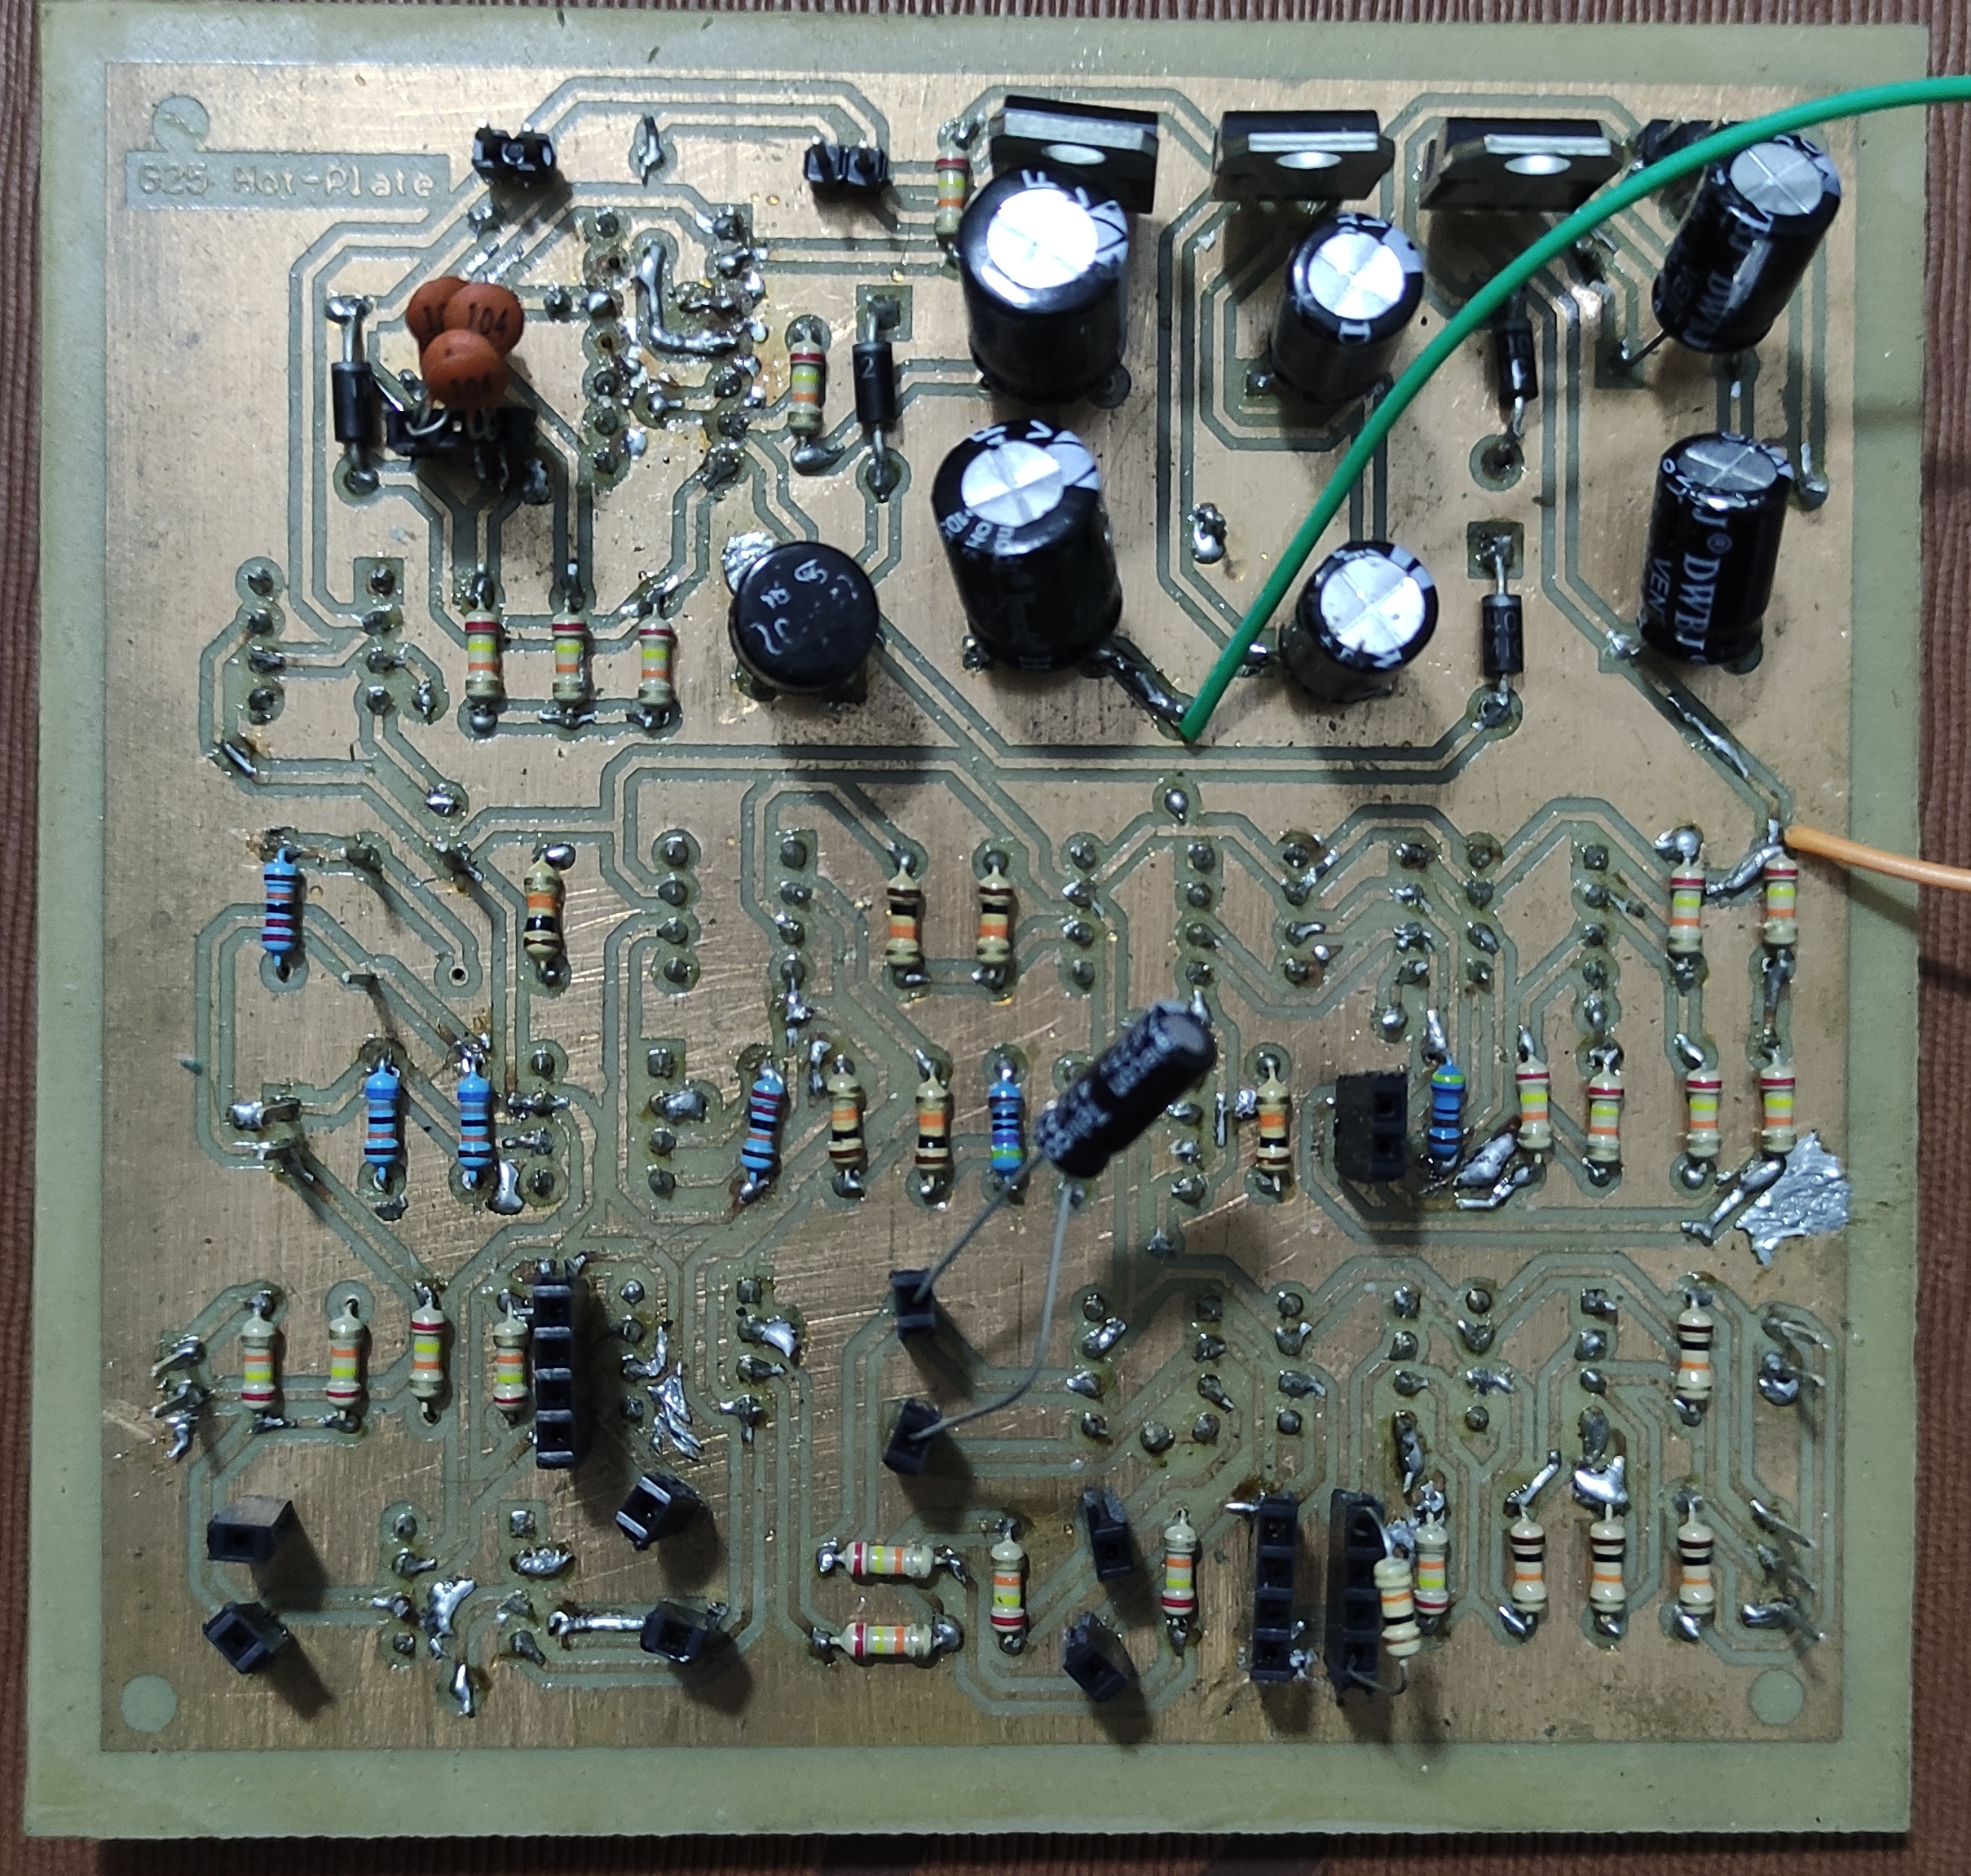
\includegraphics[width=\textwidth]{PCB fabricated/pcb2.jpg}
\captionof{figure}{PCB - Top Layer}
\end{minipage}

\begin{minipage}{0.45\textwidth}
\centering
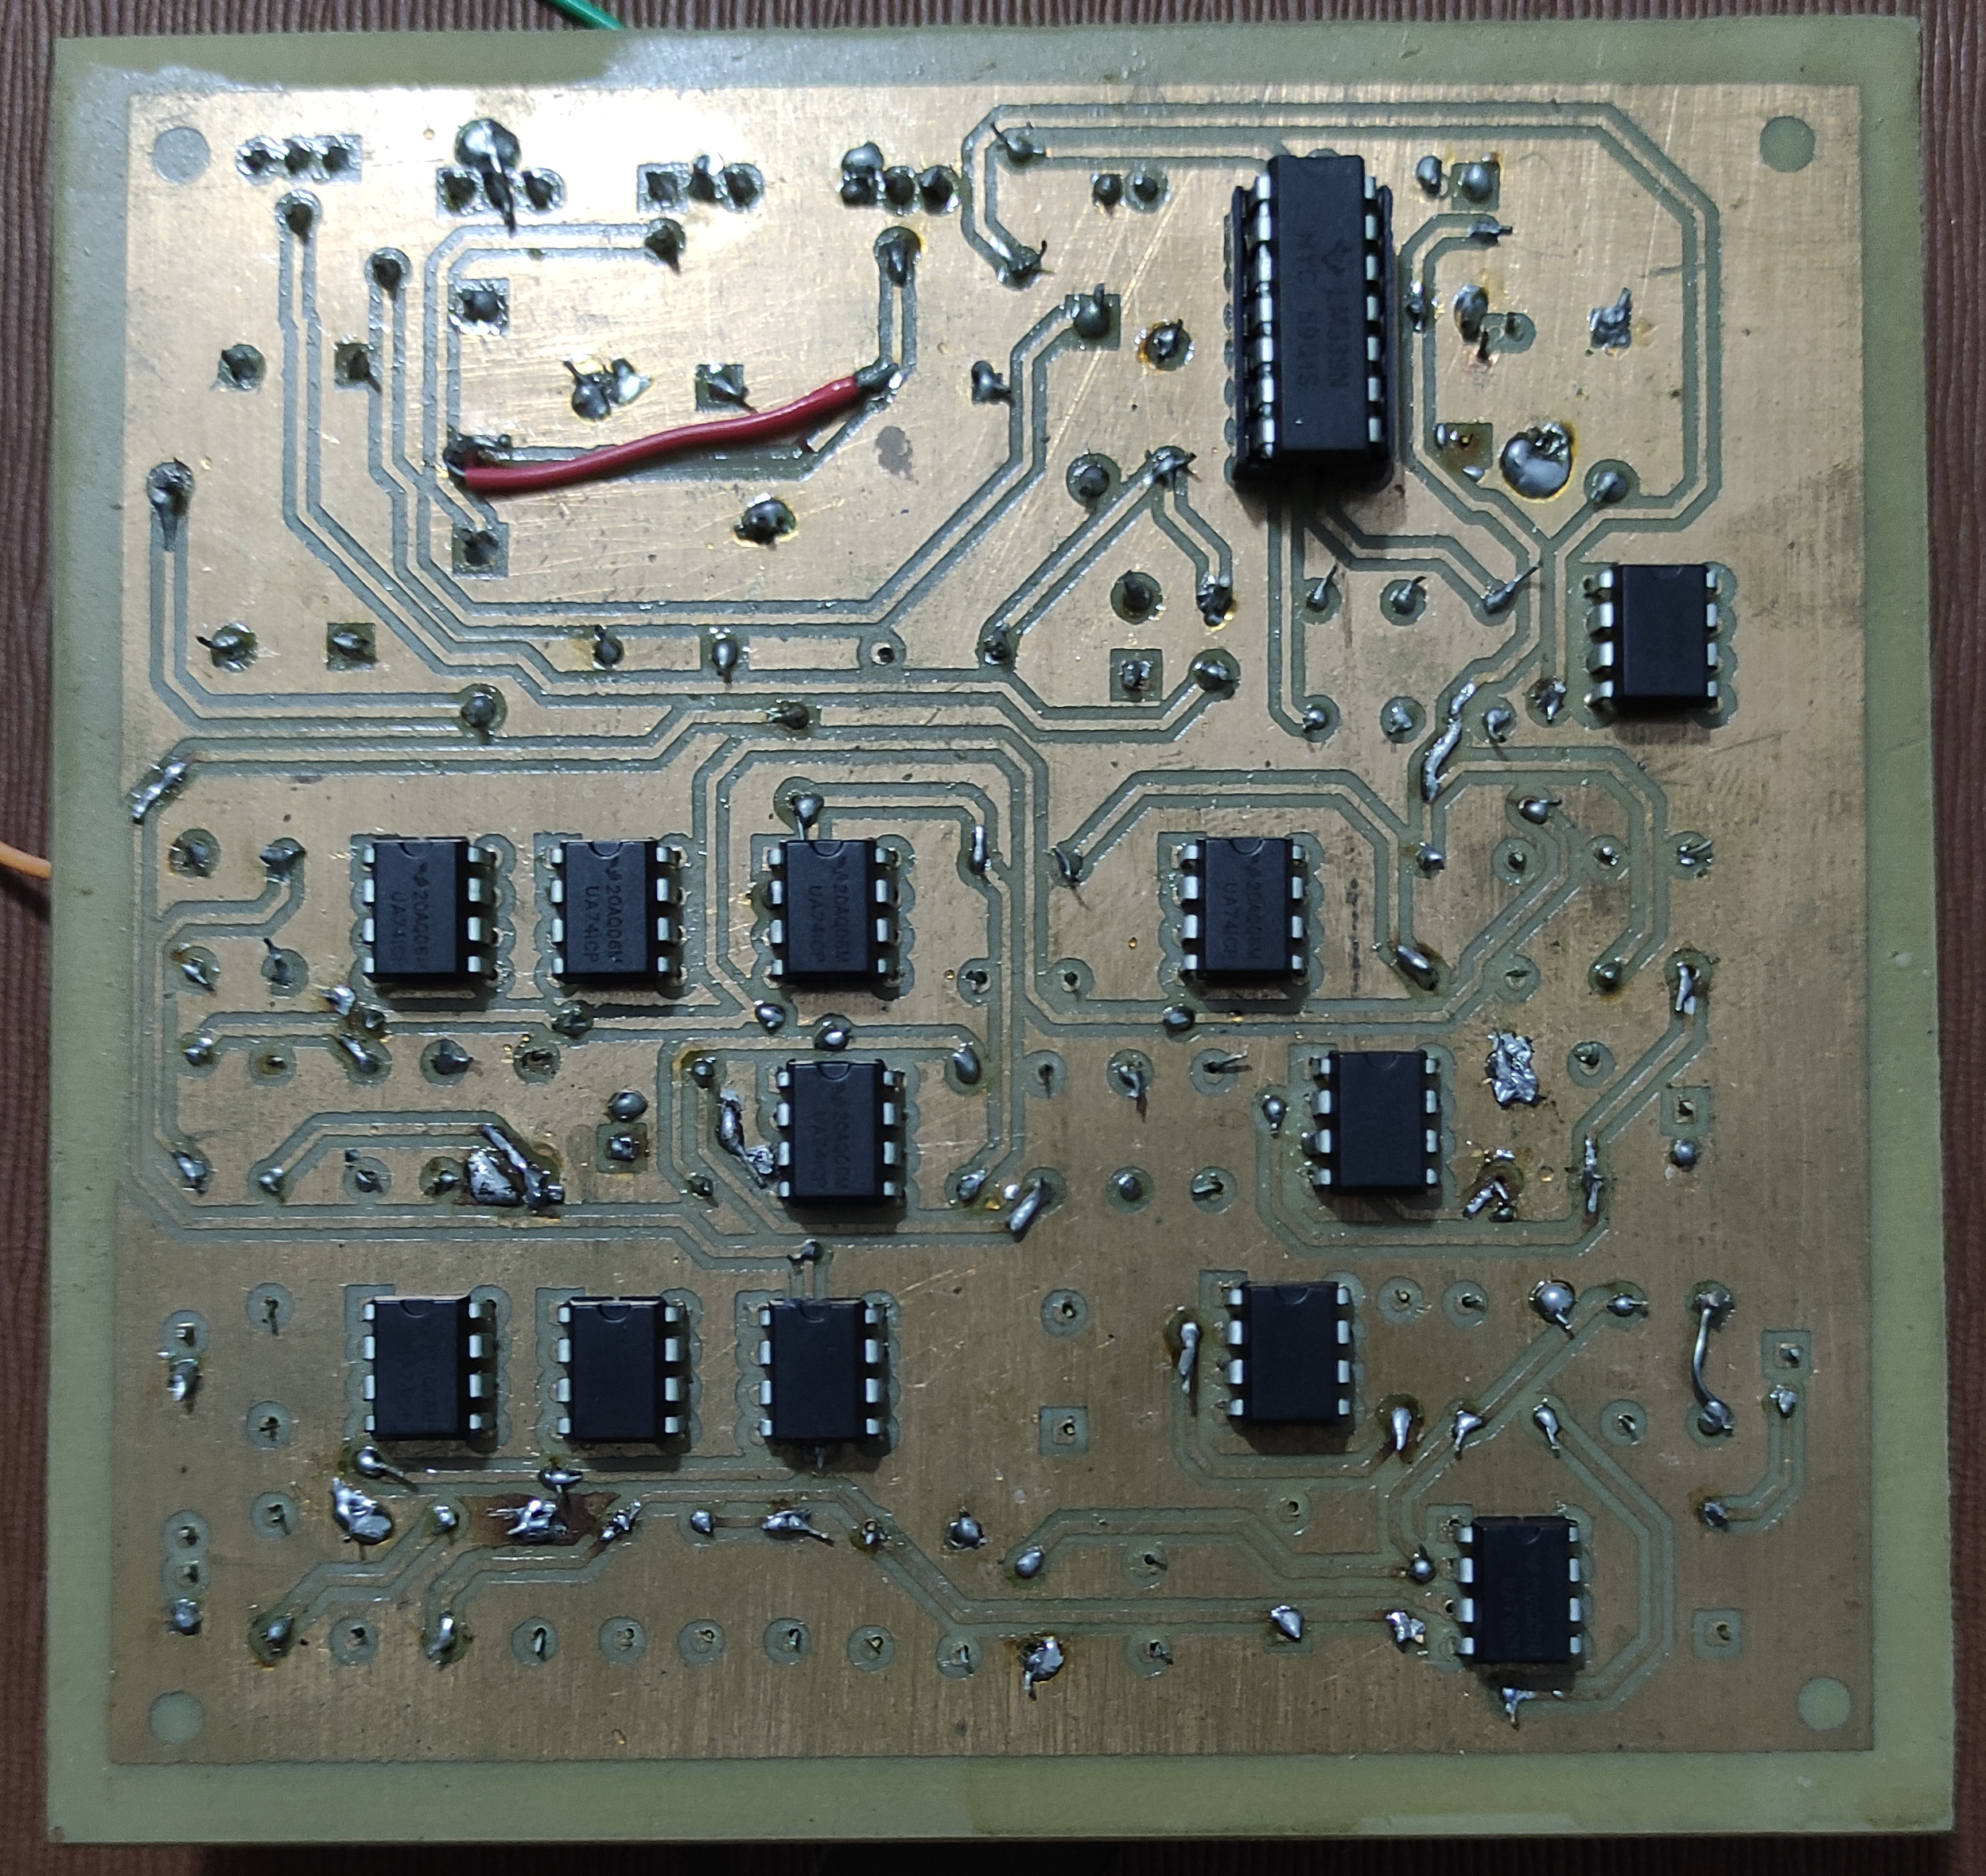
\includegraphics[width=\textwidth]{PCB fabricated/pcb1.jpg}
\captionof{figure}{PCB - Bottom Layer}
\end{minipage}

{\let\clearpage\relax \chapter{Discussion}}

The goal of our project was implementing a PID controlled hot plate which consist of proportional, integral and differential parts is widely used in controlling systems. We divided the entire circuit into six sections and worked on each other. The details of those parts are described separately above.

With the sensor interface circuit, we used an improved Howland current pump with a buffer based constant current circuit rather than a normal potential divider. The purpose of that part is to feed a sensor with a constant current less than 1mA.

The width of the PWM depends on some reasons. One of them is the capacity of the capacitor with the transistor of that circuit. Then we changed this capacity value and found the suitable value to obtain an appropriate width of the PWM.

When looking at the triac circuit, we had to experimentally find suitable resistor and capacitor which are connected to the triac. For the safety we used a heat sink to evacuate the heat from the triac.

First, we used a filament bulb instead of water heater. We examined the change of its brightness according to the given voltage value. To observe the wave form getting cut off, we had to use 12V(rms) AC input rather than using 230V(rms) AC, since the oscilloscope does not support 230V(rms) AC.

%{\let\clearpage\relax \chapter{Acknowledgement}}

\end{multicols}

\begin{center}
\begin{tabular}{ p{0.4\textwidth} p{0.6\textwidth} }
\hline
 \textbf{Name} & \textbf{Contributions} \\
 \hline
 Tharindu O.K.D 190622R  & Deisgn the PWM generating part, Design the $1mA$ constant current source,Triac Circuit, and Soldering. \\  
 Tharundi P.D. 190626HV & Altium PCB design and routing, instrumental amplification for sensor interface \\
 Tharindu O.K.D. 190622R & Enclosure Design, PID simulation design and testing, Report Diagram creation\\
 Udara A.G.N. 190636M & Report writing, PID controller testing and tuning\\

 \hline
\end{tabular}
\end{center}